
\chapter{A modular synthesis engine}

\epigraph{We can now see that the whole becomes not merely more, but
  very different from the sum of its parts.}{\emph{More is Different:
  Broken Symmetry and the Nature of the Hierarchical Structure of
  Science}\\\textsc{Philip Warren Anderson}}

\section{Analysis}

In the previous chapter we built a system for sound representation,
processing, and interfacing. In such system, interactions
between different processing elements is hard-coded in the control
flow of the program itself and the relations among the statically
parametrised types that intervene.

As described by requirements \ref{req:iter2-begin} to
\ref{req:iter2-end}, we shall develop a system where the basic DSP
units can be composed orthogonally and hierarchically to build complex
devices \emph{at runtime}. With the applications built on top of our
framework being targeted at live performances, it should be
particularly dynamic.

\subsection{An abstract model of a modular synthesiser}

In a modular synthesiser, the sound generation is made by
interconnecting basic processing units. Each of them might generate
sound, filter it, and can have a varying number of inputs and outputs
of different kinds. Because a module can apply virtually any
mathematical function to its inputs; we can realise any synthesis
technique --- i.e. additive, subtractive, FM/PM --- by just wiring the
available modules in an appropriate way.

We can characterise such a system by abstracting the parts of one of
these processing units. A hardware modular synthesiser can be used to
illustrate the concepts behind this, as shown by the \emph{frequency
  shifter}\footnote{A frequency shifter is a module that produces
  oscillating modifications on the frequency components of a given
  input signals, producing interesting Doppler effects, binaural
  effects, vibratos, and so on.} in figure \ref{fig:hwmod}. We can thus
taxonomise its parts as in the following; we will later use this
terminology in our design.

\begin{description}
\item[Input ports] These are the signals that come from another module. In
  the example figure we can see a \emph{input} signal that carries an
  arbitrary sound wave to be frequency-shifted, and a \emph{CV in},
  which is used to modulate the shift parameter. In a hardware module
  we can consider as an input anything that can go through a wire,
  thus we are no limited just to analog time-domain signals, but we
  can consider a digital MIDI input of a synthesiser as an input
  signal too.

  In our software system we are even less constrained, and our system
  should cope with signals of any kind --- i.e. of any type, in the
  programming language sense. Note also that an input might remain
  disconnected during execution of the synthesis graph, and a proper
  default behaviour should be implemented in that case.

\item[Output ports] These are the signals that the module sends to other
  modules. They are of the same nature than their input counterparts.

  In order to connect an output to an input, the kind of signals that
  flows through them must match; in a computer based digital system
  this should be checked and proper error handling must come into
  action if necessary or maybe some automatic conversion mechanism if
  safe and applicable.

  Note that while on and hardware synth inputs and outputs are
  generally related in a one-to-one manner --- unless we do not
  consider a hub/split or a mixer a module by itself but a connection
  device --- in software we can relate them in a one-to-many fashion,
  as the value produced in an \emph{output port} can be read several
  times by different modules if it has its own memory.

\item[Parameter controls] These allow the user to tune the different
  settings of the device. In a hardware device, they are most of the
  time represented by a knob or a slider, but modern synthesisers
  include bidimensional touchpads and other input devices for
  controlling the process.

  Note that, at this stage, the notion of a \emph{parameter} or
  \emph{control} is not directly related to how it might be
  represented to the user --- like a text-box, virtual knob, or
  whatosever --- but to the abstractions that the a DSP module uses to
  get input from outside of its inner processing function. Just like
  an input port, it should be of any type. For example, any control
  that is naturally representable with a knob or slide is quite often
  a \emph{float} parameter.

  The reader might wonder how is this different from an input port in
  a software system. On the one hand, controls do not have any
  built-in interconnection system. On the other hand, the
  synchronisation mechanisms used to pass the values through controls
  and ports are quite different. This is so because while the
  information that goes through ports is to be used only by the DSP
  modules, controls get input from the user interface thread, thus
  requiring special care. We will discuss this further in the next
  section.

\item[Status controls] These provide feedback to the user about
  relevant parts of the state of the processing. In the example
  figure, a red led is light up when the output signal exceeds the
  \emph{clipping value} --- i.e. the upper threshold of the admissible
  range of the amplitude of the signal --- suggesting the user to
  lower the gain to avoid annoying distortion. Everything that have
  been said about parameter control applies here. Once again, what is
  important is the abstraction not the visual representation; those
  the aforementioned example would be a \emph{boolean} status control in our
  system, that might be represented by any other means.
\end{description}

\begin{figure}
  \centering
  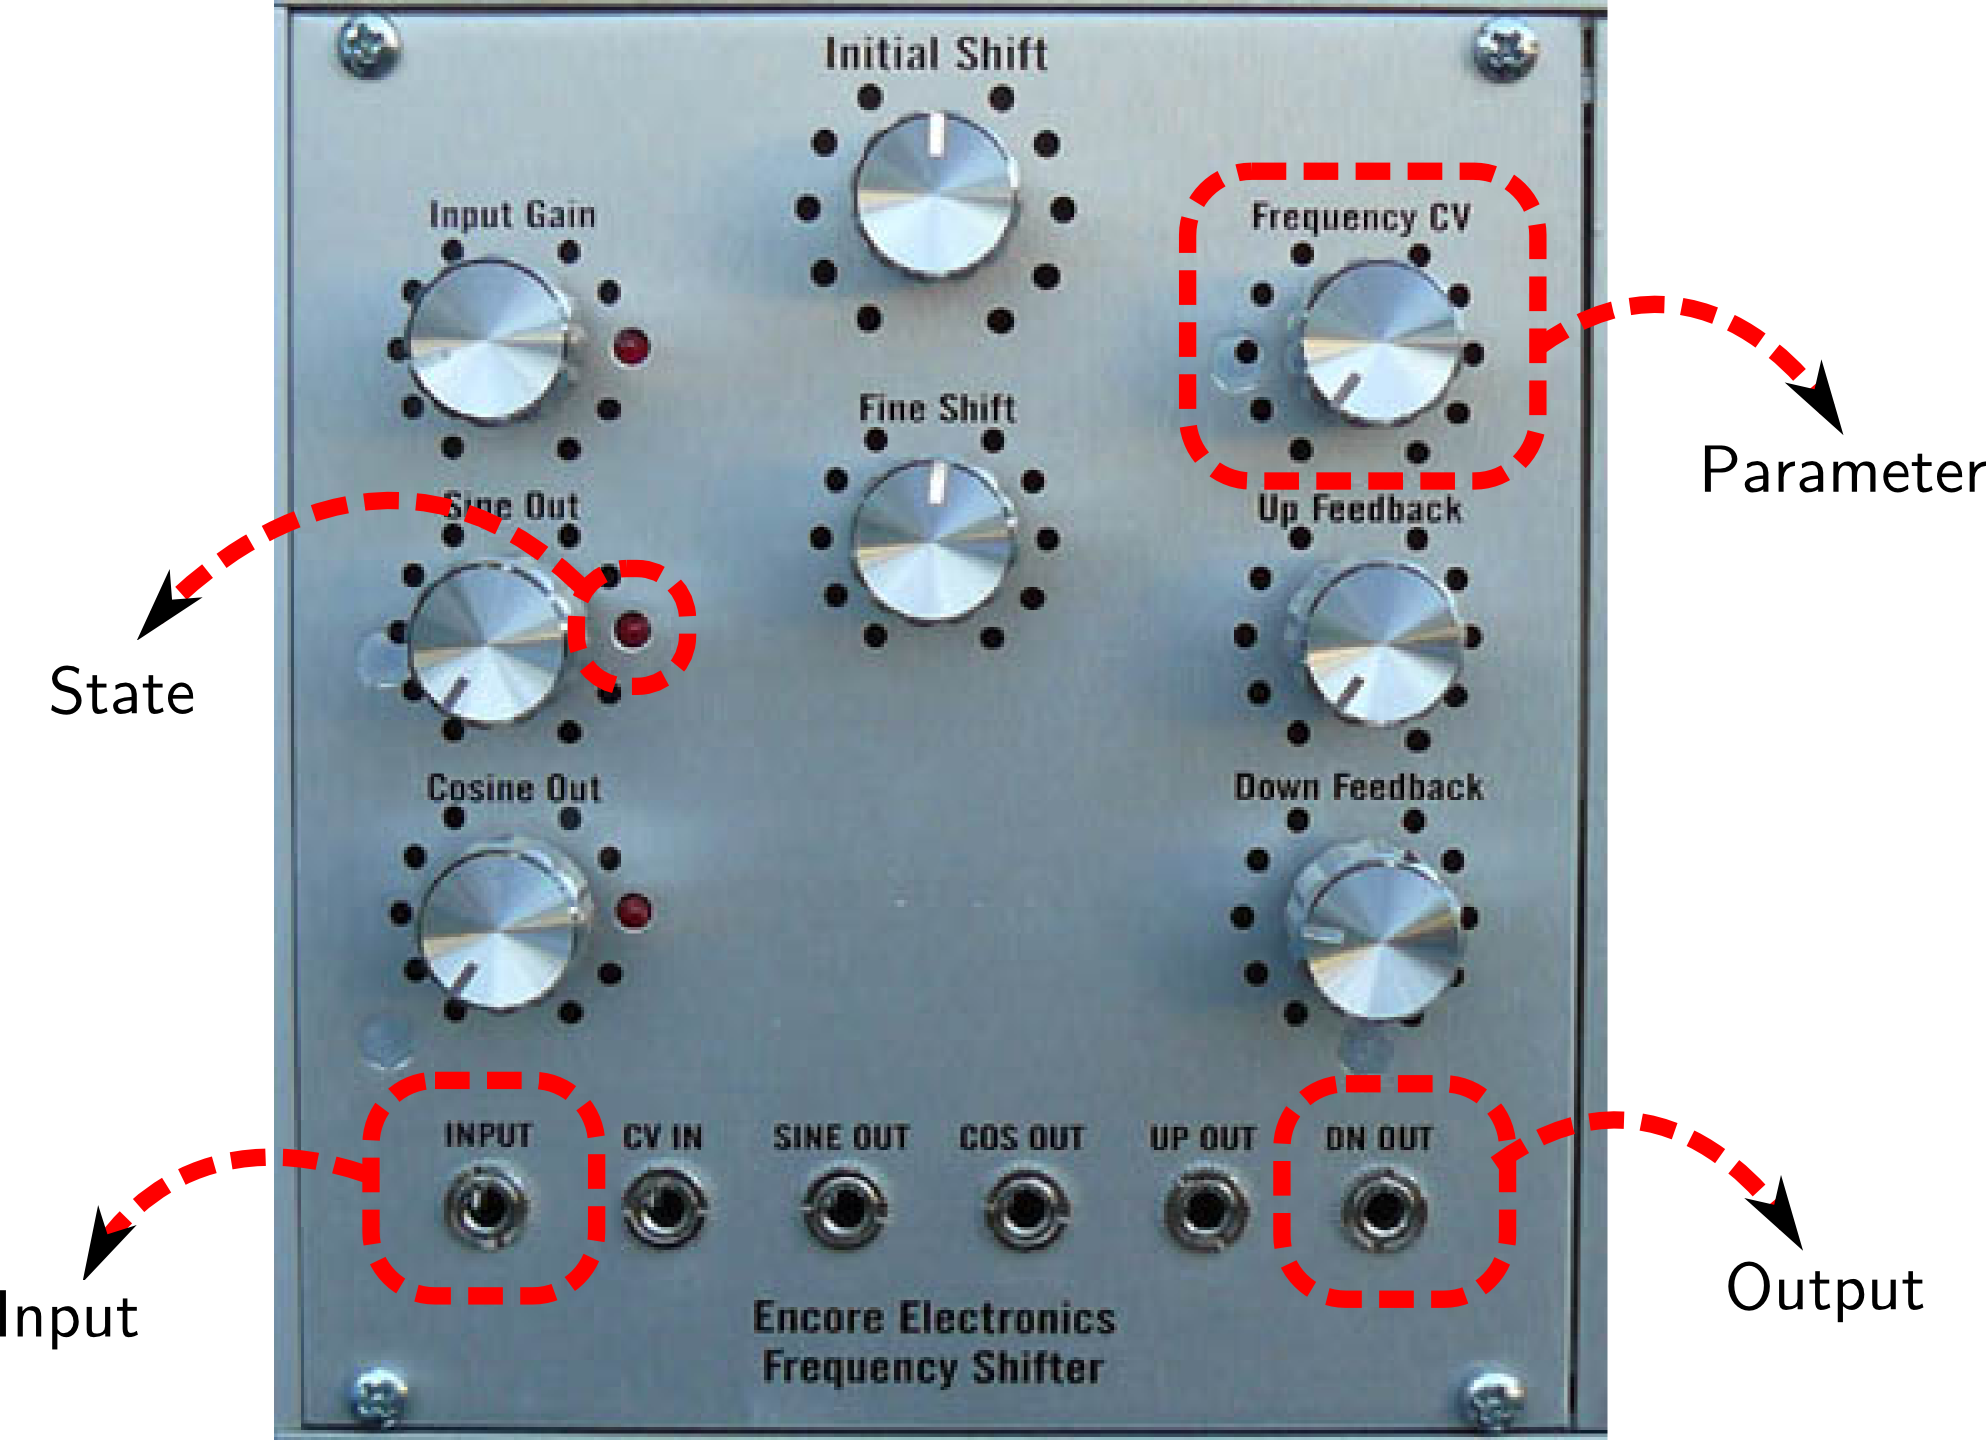
\includegraphics[width=.9\textwidth]{pic/hwmod.png}
  \caption{Components of a synthesis module illustrated in a standard
    \emph{frequency shifter}.}
  \label{fig:hwmod}
\end{figure}

A collection of modules and the connections among them is called a
\emph{patch}. In a hardware modular synthesiser, these are assembled
in special racks that have slots satisfying some standard to place the
modules in them --- for example, the module in the figure fits in
\emph{eurorack} slots. In many software synths, and specifically in
the one we are developing, patches can be arranged hierarchically. We
can visualise this as if we could put a whole rack into a black box
with holes to expose certain controls and ports to the outside, and
then place this box in a larger rack. This is very useful in a
software synthesiser; for example, one could build a complex patch out
of low-level processing primitives and expose a simplified
interface. Some software, like Reaktor, call these patches
\emph{instruments}. This arrangement can then be stored into a file
for later use. On the Internet one can find many collections of these
ready-to-use patches, and there are even commercial packages developed
by professional sound designers.

The \emph{conceptual class diagram} in figure \ref{fig:graphconcept}
summarises all this. Note that this is a conceptual class diagram, not
a design one, so there is not necessarily a direct match to the
classes in the actual code, not even terminologically.

\begin{figure}[h]
  \centering
  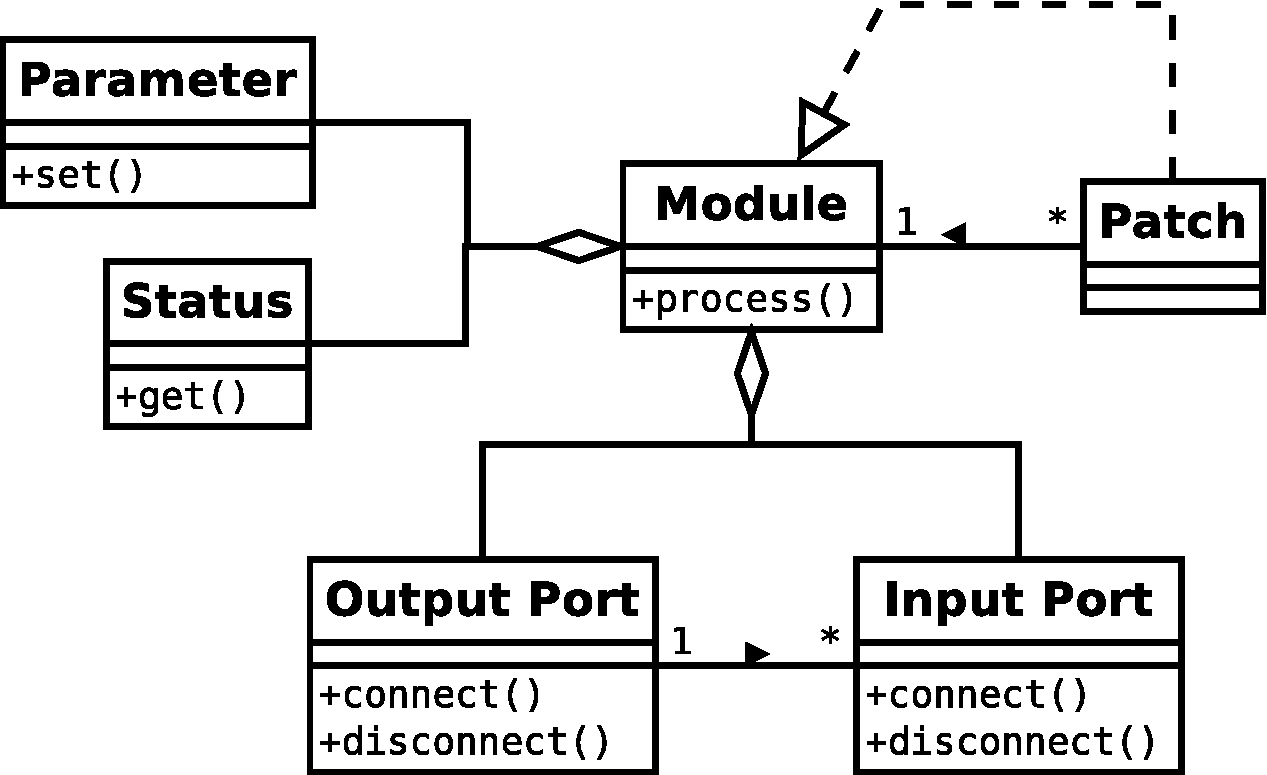
\includegraphics[width=.9\textwidth]{pic/graph-concept.pdf}
  \caption{Conceptual class diagram of the modular synthesis main entities.}
  \label{fig:graphconcept}
\end{figure}

\subsection{Software real time synthesis concerns}
\label{sec:rtsynth}

Our system generates the audio in real-time sending it directly to an
output device --- a sound-card. Even more, it is specially targeted at
live performances, so every operation should be designed such that it
does not disrupt the audio generation process and generates no kind of
noise. For example, in some software modular synths changing a
connection among ports triggers a recomputation of the dependencies
among modules to generate a compiled form of the patch for easier
execution; but that often that takes long enough to produce a small
buffer underrun --- i.e. an audible click --- as it might involve
doing non-linear computations or locking certain mutexes to
synchronise the state with the user thread. Actually, the port
reconnection issue requires special care, as we will discuss in
section \ref{sec:modports}. Because of \emph{dynamic-patching} we
should expect the topology of the synthesis graph to change a lot
during a live performance.

To better understand this problem we should understand how audio is
usually processed in real-time, thus feeding us with proper
terminology and knowledge to later tackle the issue. While this might
seem like a design issue to some, this is such a universal structure
that it shall be consider as a fixed constraint to be analysed than a
design decision itself.

Ideally, we would produce each sample one at a time and send it to the
output device. However, because we have to produce, at least, 44100
samples per second --- more in some professional applications ---
traversing all the synthesis system for every frame involves many
function calls, some of them even require dynamic dispatch in an
extensible system like ours, leading to a too low performance to
deliver the samples on time. For this reason, audio is processed
blocks of \emph{block size} samples in tight loops. This \emph{block
  size} might match the device's buffer size or it might be
smaller. Parameter and status values are updated only in between
blocks. Thus, we should try to keep the block size as low as possible
to avoid noticeable latency, and most professional audio software
allow changing this parameter to fit the machine processing power. A
sensible block size is 64 samples, like Pure Data's default. Using the
terminology in \cite{boulanger10audio}, we can distinguish between
\emph{audio rate} --- i.e. the frame rate as described in the previous
chapter --- and \emph{control rate}, which is the sampling frequency
of control signals --- i.e. the signals that produce only one sample
per processing block:

\begin{equation}
  control\_rate = \frac{audio\_rate}{block\_size}  
\end{equation}

Note that control signals are not restricted to what we labelled as
\emph{controls} in the previous sections. In fact, through a
\emph{port} may flow signals at audio rate if their signal type is
that of an audio buffer that holds a block of samples, or at control
rate if their signal type is that of a single sample, like a
\type{float} or \type{double}.

Interleaving the sound generation within the user-interface loop is
not plausible; thus the audio processing lives in its own thread/s. In
fact, as we saw in the last chapter, some audio output interfaces like
Jackd control the audio thread themselves invoking the processing
function through a callback. Our own device API wrapper that we
developed in the previous chapter promotes this kind of asynchronous
output and simulate it whenever the output system only provides a
blocking I/O interface. The inverse of the control rate, that we may
call the \emph{control period}, provides a very explicit deadline for
the block processing function. Missing the deadline might not kill
people, but it would produce an unpleasant clicking noise and thus we
have to do as much as possible to meet the deadline\footnote{In fact,
  in the middle of a live performance with a $10^5$ watts sound
  system, consequences might be more severe as it seems superficially
  :)}. Our system can be categorised as \emph{soft real-time}
\cite{tanenbaum07mos}. Apart from trying to get real-time priority in
the audio thread, we have to take special care when developing the
program, and this will deeply influence the design:

\begin{enumerate}

\item Avoid system calls in the audio thread. System calls produce a
  context switch and it can take quite long until the audio thread is
  preempted back; at least too much to meet the deadline. This is
  specially true for I/O system calls. In the previous chapter we
  already provided some devices to avoid this problem, like the
  caching file readers.

\item Avoid contending for a \emph{mutex} or some other kind of lock
  with the user thread. Without special support from the operating
  system --- like priority inheriting mutexes --- this can lead to
  priority inversion \cite{kim03basic}. Even in the later case, the
  context switch produced by the contention gives good chances to miss
  the deadline until the audio thread is preempted. The overhead of
  locking a mutex when there is no contention is negligible in most
  operating systems, and it definitely is in Linux which uses
  \emph{futexes} (Fast User-space Mutex) to implement them
  \cite{franke02futex}, so using a \emph{try-lock} operation is
  usually acceptable. The rule of thumb is to never wait on a mutex in
  the audio thread, and use lock-free data structures
  \cite{valois96lockfree} or do conditional locking instead.

\item Because the dead line depends directly on the block size $n$,
  algorithms running in the audio thread should be in $O(n)$. A special
  consequence of this restriction is that allocating memory in the
  heap, at least with the default allocator --- i.e. using \type{new}
  --- is forbidden. This is so because memory allocation algorithms
  are not proportional to the size of the requested block, but instead
  depend on non-deterministic properties like the pattern of memory
  usage and use complex search algorithms to find a fitting block of
  spare memory. This restriction implies that manipulating STL
  containers is forbidden too. For some special kinds of objects, like
  same-sized objects, a custom memory allocator can do the job
  \cite{alexandrescu01modern}. Sometimes, an intrusive data structure,
  like \emph{Boost.Intrusive} STL counterparts
  \footnote{\url{http://www.boost.org/doc/libs/release/doc/html/intrusive.html}}
  are enough to avoid the allocations. In other situations, we can
  release the job of allocating memory to the user thread, use custom
  data structures or any ad-hoc solution.
\end{enumerate}

\subsection{Anticipating future needs}

For the sake of proper workload balancing, several features that
deeply affect the structure of this layer are delayed for later
development iterations. However, to prevent rewriting the code at
those stages, we should anticipate what characteristics are
required from the basic constructs in order to later extend the system
with such features.

\subsubsection{Polyphony}

Polyphonic audio allows building chords and enrich the whole harmonic
depth of the music \cite{johnson02measured}. Polyphony is produced
when several notes are played at the same time; for example, by
pressing simultaneously several keys of a keyboard. Actually,
polyphony is also present without simultaneously pressing several
keys, as instruments usually have a significant \emph{decay time} ---
i.e. the time between the key release and the sound fully fades out
--- blending the sounds of successive key strokes.

Because in a modular synthesiser a generator is producing a single
tone at a time, it is not trivial to implement polyphony. In practice,
several copies of the processing graph are to be maintained, each one
is called a \emph{voice}. When a new note is to be played, the system
has to allocate a voice for it and trigger the processing; when it did
fully turn off the voice is released. Voice allocation is in many ways
similar to other allocation mechanisms, like page allocation in an
operating system, and different stragies have been proposed:
\emph{round-robin}, \emph{last-in-first-out}, \emph{priority based
  algorithms}, etc. The number of of voices is called the \emph{level
  of polyphony}, which is usually user-controllable but fixed during a
performance parameter of the system. In practice, modern computers
allow levels of polyphony high enough (from 16 to 128) such that the
sophistication of the allocation mechanism is not relevant for the
overall qualitative experience of the overall sound produced by the
synthesiser. Also, in a modular software synthesis engine, a whole
network needn't be polyphonic. For example, some dynamic range
compression or reverb filters are usually applied to the final mixed
sound of all voices, yielding better performance but also a richer
sound.

It is not worth to concentrate on the actual management of the
different voices and the triggering mechanisms until sequencing and or
MIDI support is developed in later stages. However, there are some
questions that we do have to address now:

\begin{itemize}
\item We have to split the responsibilities of the different classes
properly predicting which classes will need to be extended, preferably
via inheritance, to provide the polyphony support.

\item We have to define, at least partially, an interface that
  polyphony enabled DSP nodes will have to implement.
\end{itemize}

\subsubsection{Plug-in system}

At a later stage, we plan to implement a plug-in system as defined by
requirements \ref{req:iter3-begin} to \ref{req:iter3-end}. These
plug-ins shall be in several formats, like LV2, LADSPA, or our own
defined interface. We should take this in several ways:

\begin{enumerate}
\item For consistency, the interface that we will define in this
  chapter shall be the same that our own plug-ins will implement
  later. The only significant difference should be the linking method
  of the code and the registration mechanism.

\item Object construction, even for statically linked DSP modules,
  should be done in an indirect way, via object \emph{factories}
  \cite{gamma95design}. Thanks to this, the system can later be
  transparently extended by modifying the factory object to delegate
  the construction of specially-identified objects --- objects
  identified by a resource URI \cite{mealling02rfc3305} --- to a plug-in
  loader.

\item Parameters, states, inputs and outputs of an object should
  accessed via dynamic means of introspection. In practise, they
  should be identified by strings ands modules should provide some way
  of iterating through them. Ideally, there should be some hooks to
  provide some meta-data that can be useful for an automatic user
  interface builder; for example, a parameter's range, whether it is
  naturally linear or logarithmic, etc.
\end{enumerate}

\section{Design}

\subsection{Overview}

Figure \ref{fig:graphoverview} shows an overview of the most important
classes in this layer from the musical point of view. Most of the code
implementing these classes lives in the \type{psynth::graph}
namespace, representing the fact that this layer implements the notion
of sound processing described a graph on interconnected processing
modules. The \type{node} class is the base class of all kinds of
vertexes in this graph. Therefore, \emph{node} is a synonym for what
we called \emph{module} or \emph{DSP node} in the analysis section;
i.e. it is the basic unit that processes some input signals producing
new output values. In the rest of this chapter, unless otherwise
stated in its close context, we will use the term node with this
meaning.\footnote{Indeed, we prefer this term as the name
  \emph{module} has a different specific meaning in the code, similar
  to that of \emph{translation unit}, as we describe in the
  ``Programmer guide'' addendum.}

\begin{figure}[h]
  \centering
  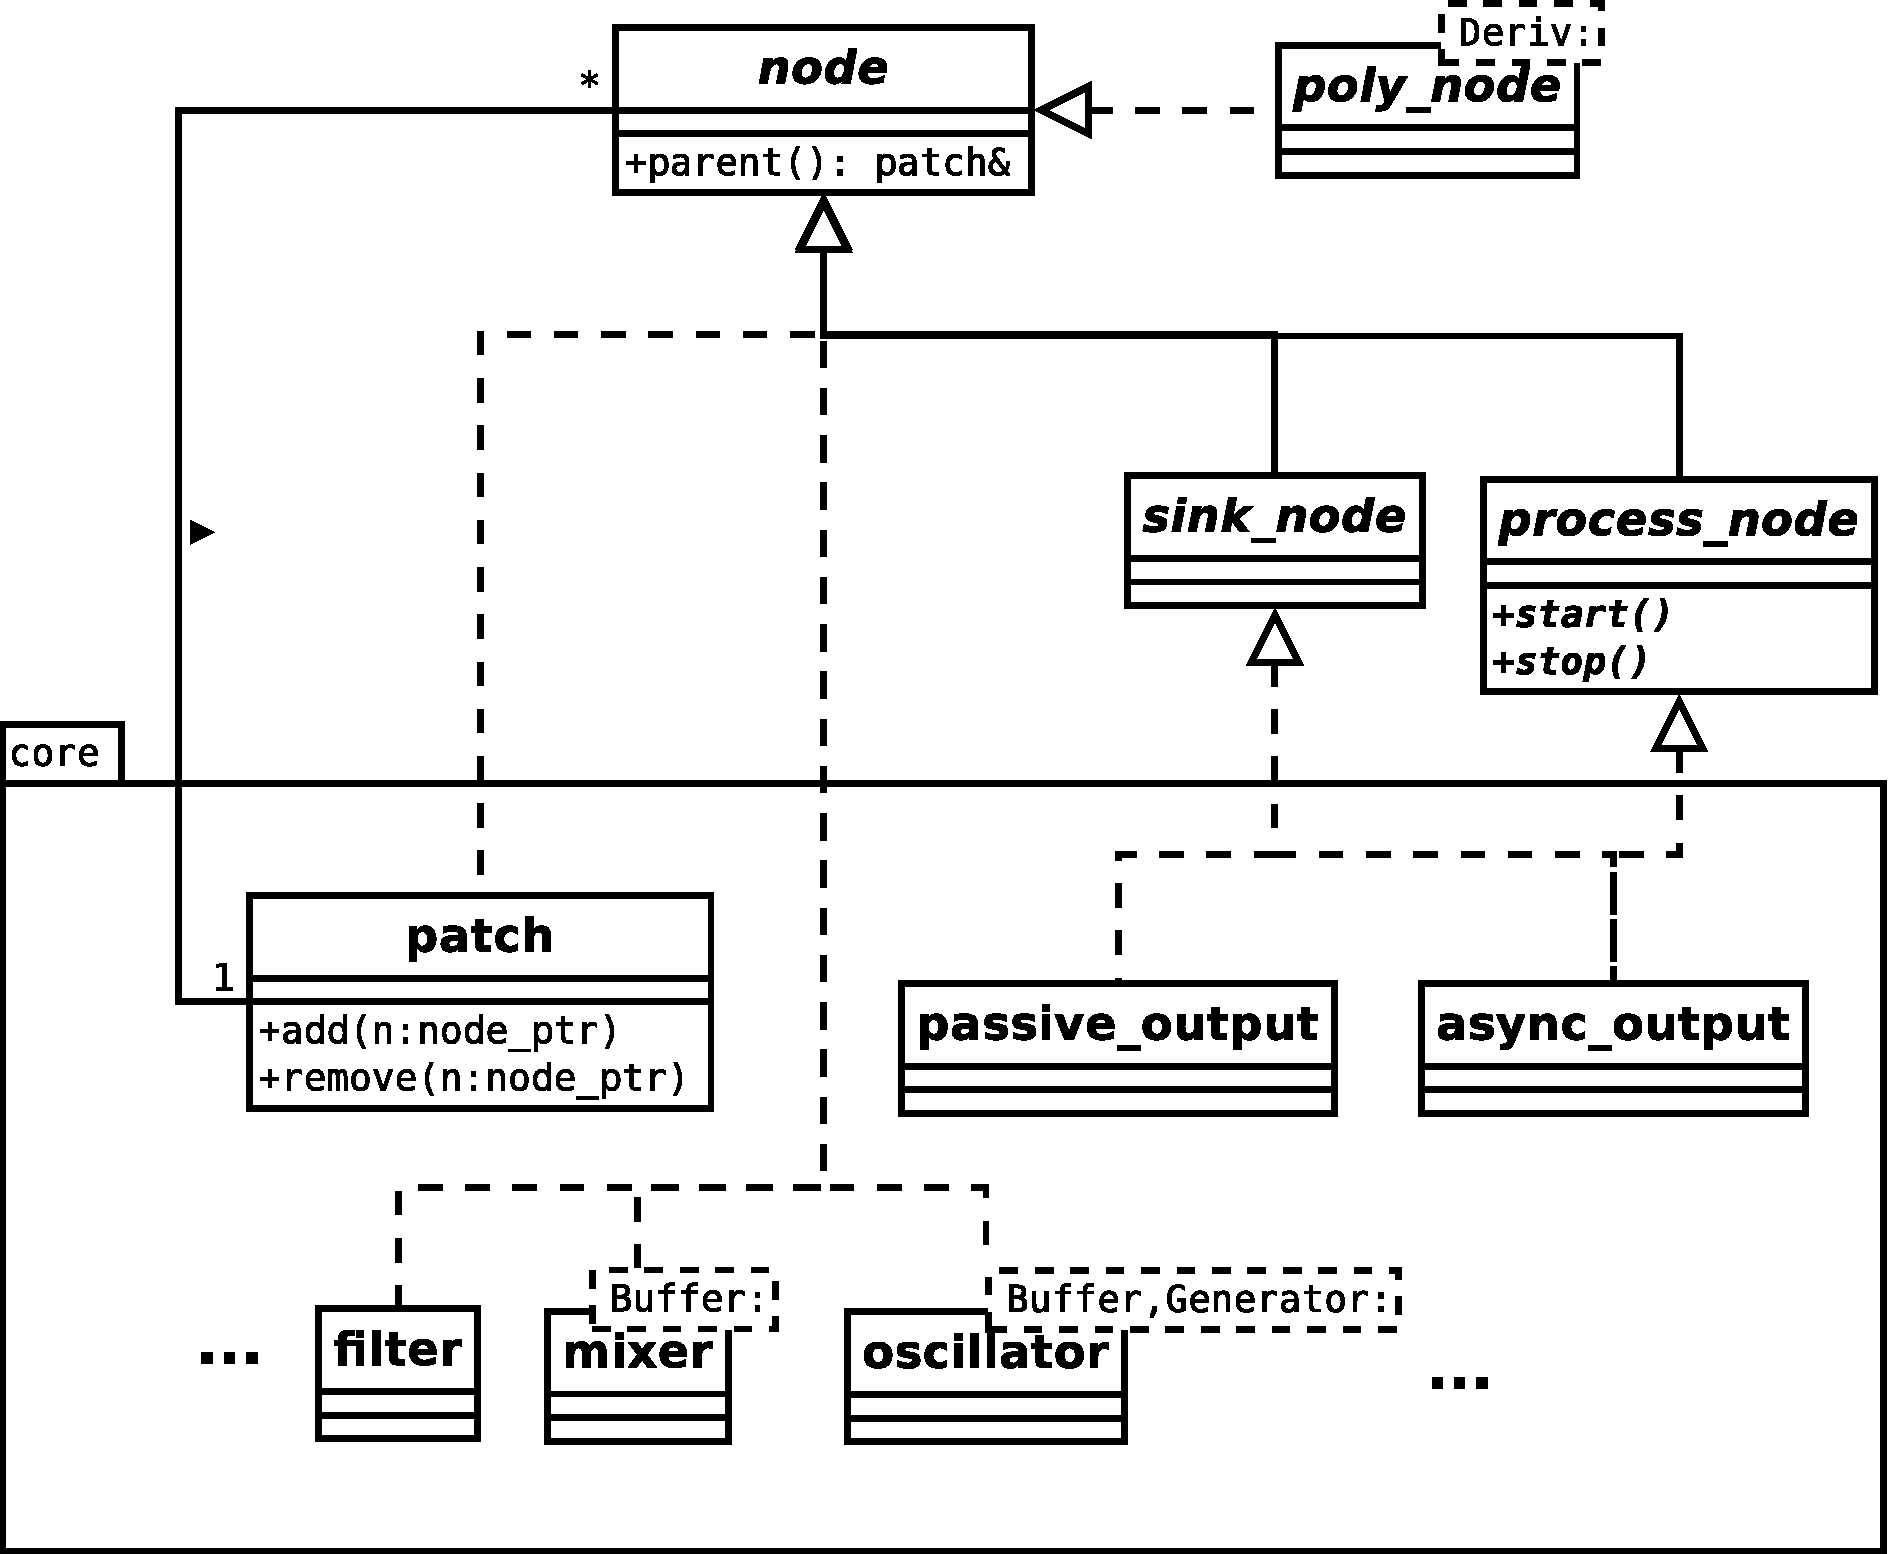
\includegraphics[width=\textwidth]{pic/graph-node.pdf}
  \caption{Overview of the graph layer}
  \label{fig:graphoverview}
\end{figure}

The \type{psynth::graph::core} namespace contains the \emph{concrete}
nodes that are implemented in our library. All these shall be
registered in the object factory that we will describe in section
\ref{sec:graphfactory} and most of the code should not instantiate
these modules directly. This introduces the notion of \emph{core
  node}, i.e. a node that is built-in --- statically linked --- inside
the library, thus is not a plug-in. Other sorts of abstract nodes that
are there only to offer certain functionality should live directly in
the \type{psynth::graph} namespace as they are considered basic
infrastructure and may be useful in the implementation of plug-ins.

We will explain other parts of this diagram later. What should be
clear now is the relationship between a \type{node} and a
\type{patch}. This is an instance of the \emph{composite} design
pattern \cite{gamma95design, vlissides98pattern}. A \emph{patch} is a
collection of nodes but it is a node by itself, building tree-like
structures that most of the time have non-patch nodes as leafs, and a
patch on its root. To ease memory management, \type{node\_ptr} is an
alias for \type{std::shared\_ptr<node>}\footnote{This is a recurring
  pattern, also explained in the ``Programmer guide''}. A node keeps a
weak reference to its parent easing traversal and some special
operations, accessible via the \type{parent ()} method.

We will next explain the execution model of the synthesis network
defined by these classes, but first, lets make a parenthesis to
explain a novel data-structure that is deep in its core.

\subsection{Heterogeneous deques --- bridging polymorphism and
  real-time processing}

As we explained in the analysis section, avoiding heap allocation is
crucial in real-time processes. Proper runtime polymorphism is said to
require heap allocation because the code paths in charge of managing
the lifetime of some object do not know its full type --- specially
the actual object size --- and thus the object can not be allocated in
the stack. While true in general, we can constrain the problem in
several ways to obtain $O (1)$ allocations if the programming language
provides enough low level constructs to implement these solutions.

A possible solution is to override the operator \type{new} for certain
types to provide constant-time allocation. Alexandrescu provides a
clever way of doing this here \cite{alexandrescu01modern}. This,
however, have several problems:

\begin{enumerate}
\item \emph{Concurrency}. We have, in general, several threads
  creating objects of these kinds. Alexandrescu solves the problem by
  using mutexes. This is forbidden in our real-time thread; which is
  just what we are trying to avoid. Maybe a lock-free data-structure
  could be used to allocate this memory, solving the issue, but we do
  not know about it.

\item \emph{Explicitness}. We would like to easily know what
  operations are safe to be performed in the real-time thread. Any
  programmer should get worried when he reads something like this in a
  real-time code path:
  \begin{lstlisting}
    some_type* x = new some_concrete_type (...)
  \end{lstlisting}
  To regain confidence about the correctness
  of that code, he should go and read the implementation of
  \type{some\_\-concrete\_\-type} and discover that it has an
  overloaded operator \type{new}.
\end{enumerate}

Another plausible solution is to constrain the set of types acceptable
in some variable. By doing so we are, in fact, changing the open world
assumption of universal polymorphism by the closed-world assumption of
ad-hoc polymorphism. Thanks to this constrain, we can, via template
metaprogramming or the new C++11 \texttt{constexpr} facility, compute
at compile time the maximum storage needed to hold values of any of
those types and allocate it in the stack; then construct the objects
in this space with \emph{placement new}. This is actually how
\emph{Boost.Variant}\footnote{\url{www.boost.org/doc/html/variant.html}}
is implemented \cite{alexandrescu01unions}, and as we are depending on
Boost already, using it is quite safe in real-time code and can be a
solution when ad-hoc polymorphism is enough.

In some other cases ad-hoc polymorphism is not enough, but the pattern
of object construction and destruction can be constrained instead. We
can think of \emph{the heap} as a global data-structure --- a
data-structure that is so useful that its insertion and deletion
operations are keywords of the language itself, let them be the
operators \type{new} and \type{delete}. In fact, its interface is very
similar to that of a multi-set, but without iteration and with the
ability to hold elements of varying size. If we restrict its interface
such that elements can only be allocated and released in FIFO or
LIFO order, we get a \emph{deque}. 

\begin{lstlisting}[float=h!,caption=Example of usage of heterogeneous deques,label=lst:heteroexample]
  struct base {
      virtual void method () { std::cout << "b"; };
  };
  struct deriv : base { 
      deriv (int x = 0)      {} 
      virtual void method () { std::cout << "d"; };
  };

  hetero_deque<base> q;
  base b;
  deriv d;

  // 1. Copying
  q.push_back (b); q.push_front (d);

  // 2. Moving
  q.push_back (deriv ()); q.push_front (std::move (b))

  // 3. Constructing, even with params!
  q.push_back<base> (); q.push_front<deriv> (1);

  // Error checking
  // static_assert error: 'int' is not a subtype of 'base'
  q.push_back (1); 

  // Access is polymorphic!
  // Output: bddbbd
  for (Base& x : q)
    q.method ();
\end{lstlisting}

The class \type{psynth::\-ba\-se::\-he\-te\-ro\_de\-que<Base>} is a
cons\-tant-size deque that can hold elements of any subclass of its type
parameter \type{Base}. The concrete type of the object must be known
at insertion time for the deque to be able to allocate space for it in
its internal buffer. Actually, the data structure API offers three
ways of inserting an concrete derivate of \type{Base} into it, (1)
copying it, (2) moving it using R-value references or (3) directly
constructing it into the data-structure, using perfect forwarding to
pass the parameters. It is statically checked that the inserted
element is a subtype of \type{Base}. All this is illustrated by the
example in listing \ref{lst:heteroexample}.

The data-structure interface is similar to that of an STL deque, with
some differences. Because access is done polymorphically via a
reference of type \type{Base\&}, \type{value\_type} semantics, which
maps to \type{Base}, are slightly different than in most containers
because the actual elements are of different heterogeneous concrete
types. Also, because objects can be directly constructed inside the
data structure with arbitrary parameters, they needn't be regular in
any sense, this is, they don't have to be copy-constructible,
move-constructible, default-constructible, copyable or moveable. This
is quite convenient because classes that are designed to be used
polymorphically more often than not do not satisfy many of these
properties. The only restriction is that \type{base} should have a
virtual destructor if any of its derivates has a non-trivial
destructor.

Note that the data structure itself is not copyable, nor moveable, nor
resizeable. While this is feasible it has a slight memory overhead
and, as our current use-cases do not need it, we decided to stick to
the current simpler implementation. This is so because to be standard
compliant, an object identity --- i.e. the memory address where it
lives --- must remain constant during its livetime; in order to copy
or move it, we need to call the proper copy or move constructor, and
in the later case call the destructor of the moved object if it is to
be released \cite{cppstd}. Calling the proper copy or move operation
requires, at least, one function pointer --- or a \emph{vtable}
pointer for a box type. We already have a plan to implement this
feature using policy-based design \cite{alexandrescu01modern} such
that it does not cause an overhead to those who do not need it.

\begin{lstlisting}[float=b,caption=Header of heterogeneous deque elements,label=lst:heteroheader]
  template <class Base>
  struct header {
      header* prev;
      header* next;
      Base* access;
  };
\end{lstlisting}

The data structure is implemented by storing the objects in a constant
sized memory block organised in a circular buffer fashion.  We append
a header like the one in listing \ref{lst:heteroheader} at the
beginning of each a object. An empty header at the end of the list
allows to keep track of the beginning of the free space. The
\type{prev} and \type{next} pointers organise the data in the deque in
a doubly-linked list fashion. Even though the storage is continuous,
this is needed because the size of the objects is variable and only
known at object insertion time. The \type{access} pointer keeps a
reference to the object itself casted to \type{Base*}. This is
required because, in the presence of multiple-inheritance, the
\type{Base} part of the object might not be aligned at the beginning
of the object's layout. If we think about it, the \type{next} and
\emph{access} pointers are just a way of keeping track of the
static information that is lost in the \emph{type erasure}
that happens when adding a new element to the data structure: its
\emph{size} and the \emph{offset} to its still known attributes and
\emph{vtable}; the \type{prev} pointer just aids reverse traversal and
addition at the front.

Figure \ref{fig:heterostructure} represents an instance of the data
structure containing two objects. The \type{front} and \type{back}
pointers keep track of the first and last valid element in the
container. We can see how adding a new element that does not fit at
the end of the memory space, causes that space to be wasted ---marked
as \emph{offset} in the figure---  and the object is instead added at
the beginning of the memory block, where there is enough free space
available in this case, in a circular buffer fashion.

\begin{figure}[h!]
  \centering
  \subfloat[]{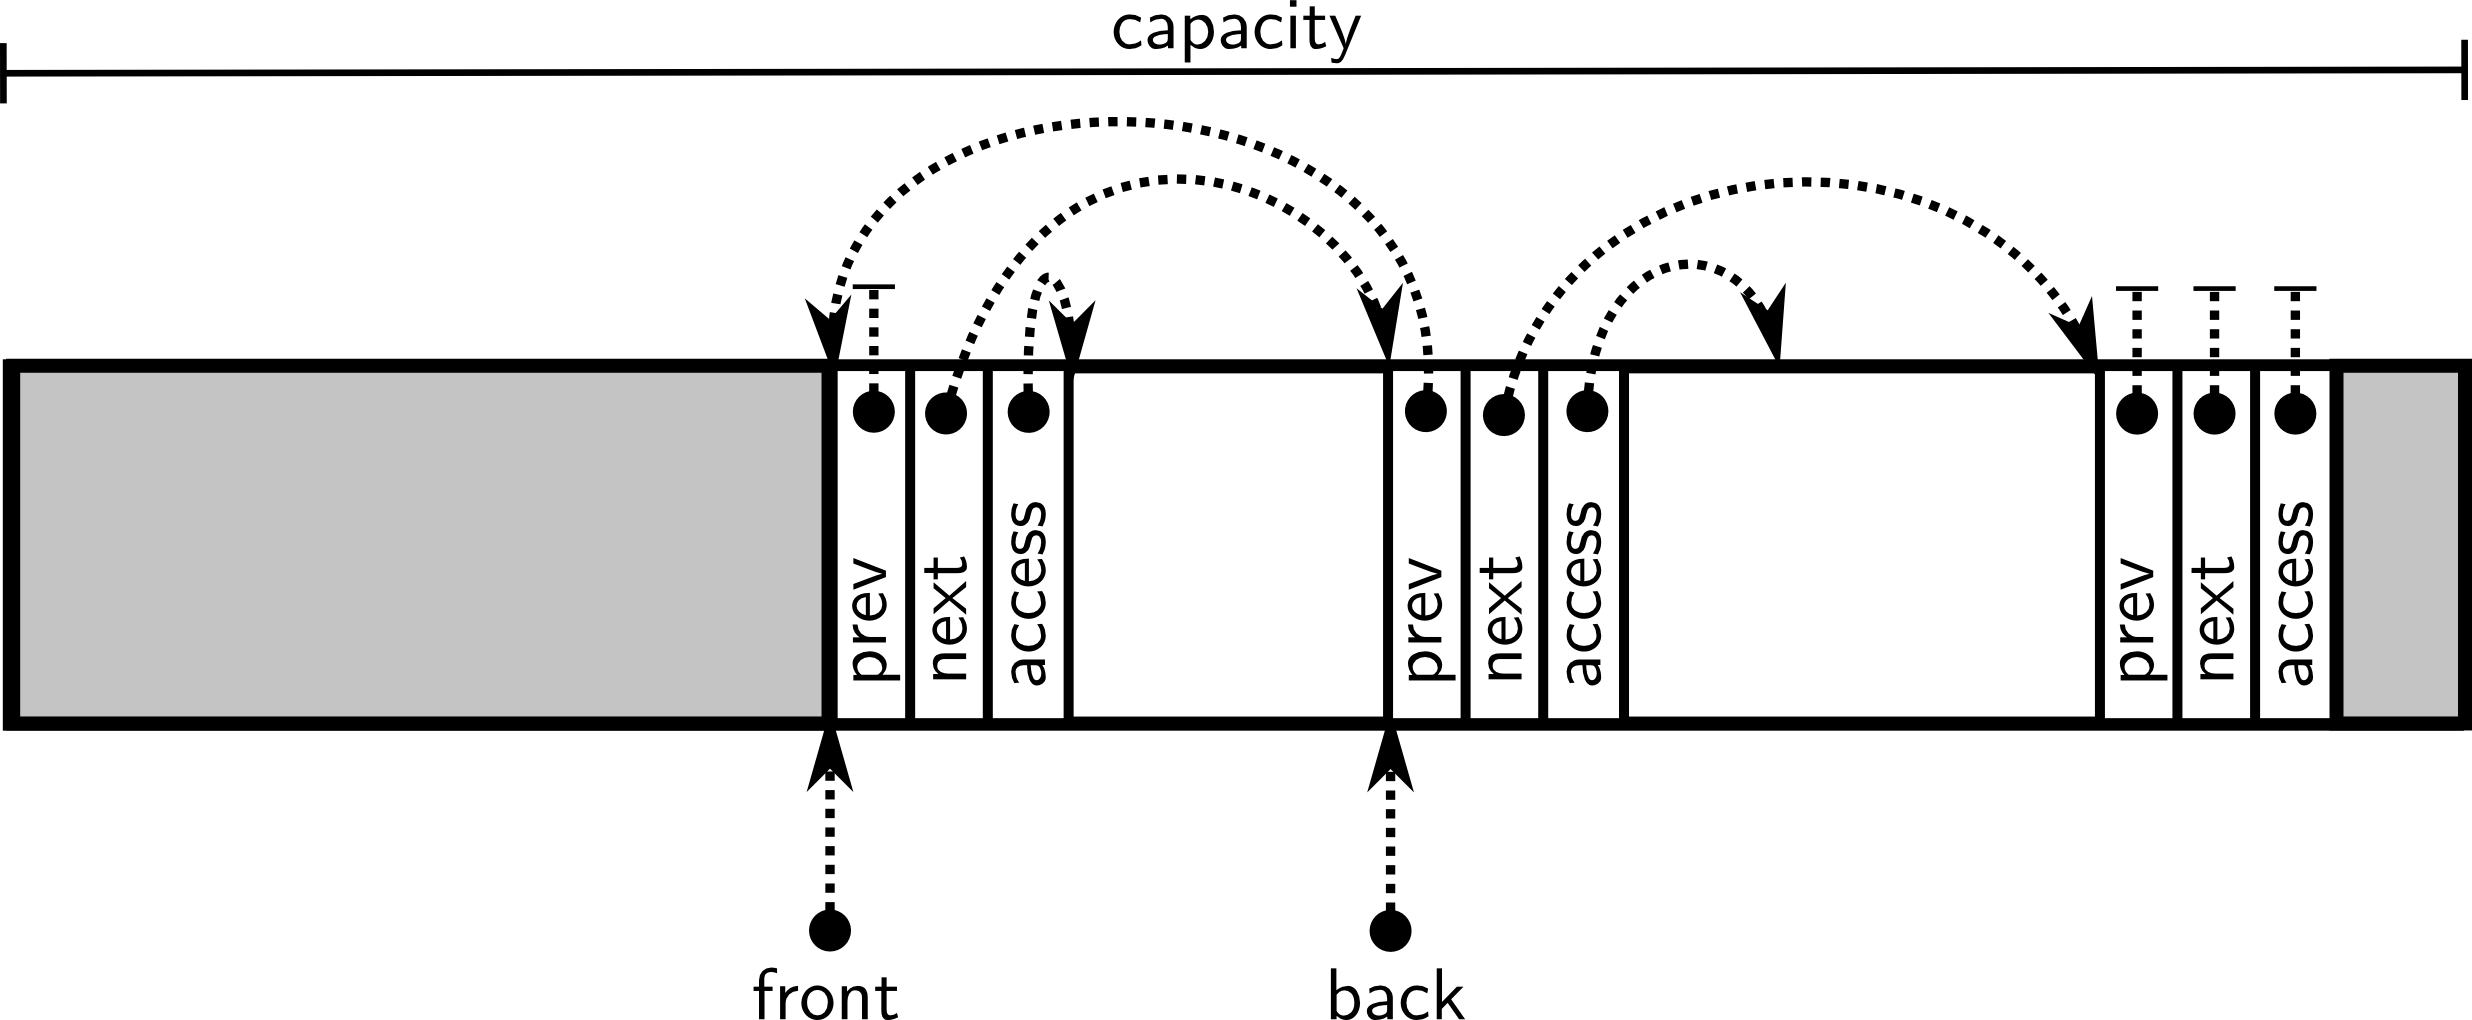
\includegraphics[width=.95\textwidth]{pic/hetero1.png}}

  \subfloat[]{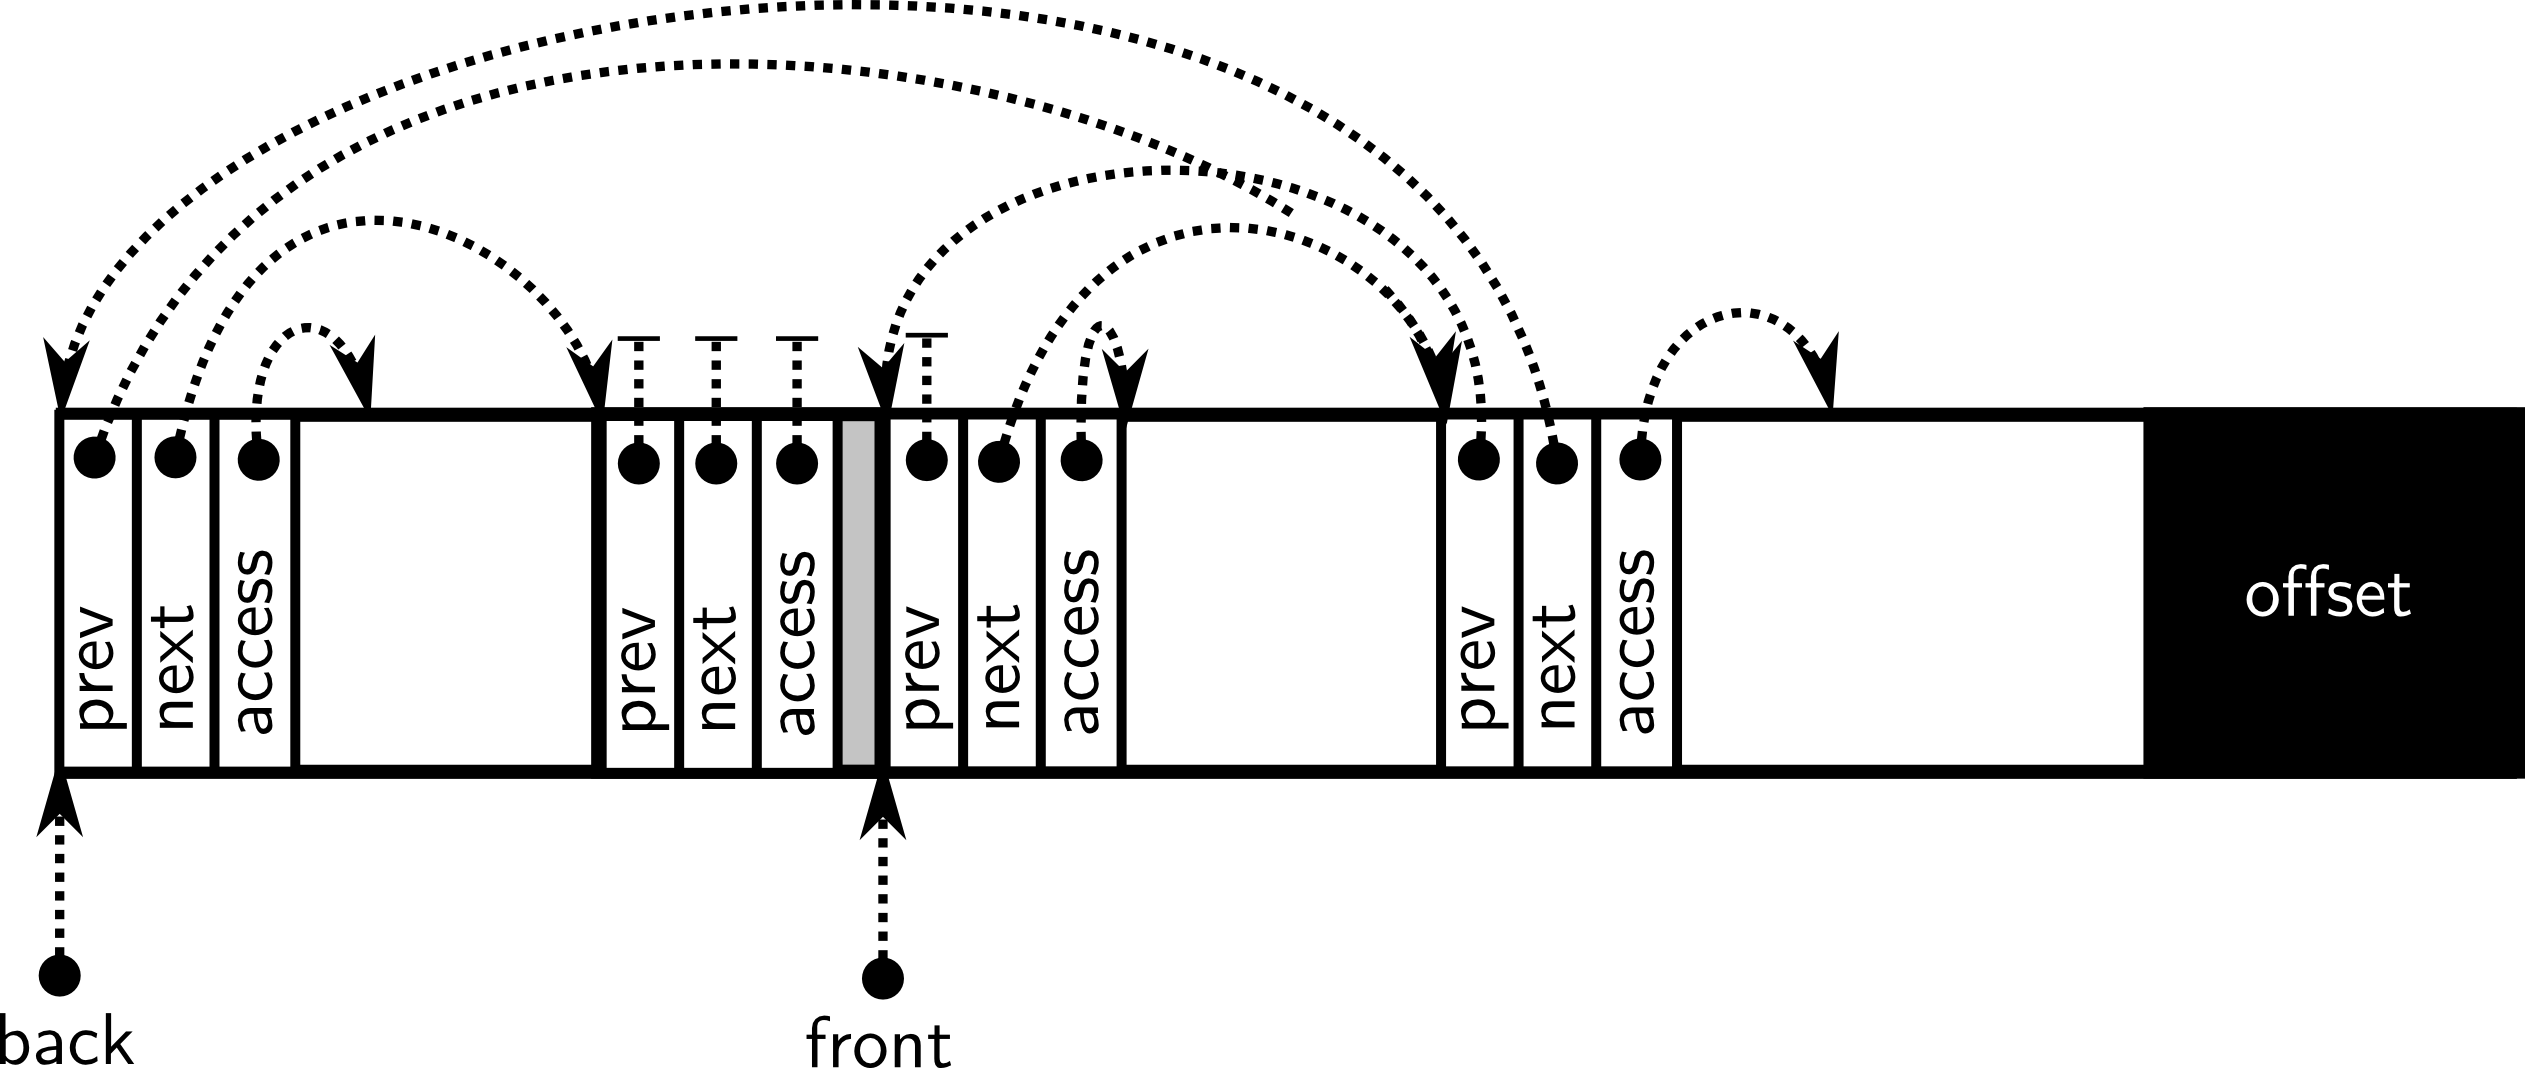
\includegraphics[width=\textwidth]{pic/hetero2.png}}

  \caption{An heterogeneous deque with two elements (a), and after
    adding a third element (b).}
  \label{fig:heterostructure}
\end{figure}

So, thanks to low level facilities provide by C++, we are able to use
different techniques to get the benefit in expressiveness and
maintainability of polymorphism in a real-time constrained
environment. Our most prominent use-case, passing active events among
different threads, gets very benefited from our last approach, as we
shall see in the rest of this section. In other parts of the system,
disjoint unions as implemented by \emph{Boost.Variant} are enough, and
we actually do use them to treat a closed family of oscillator objects
polymorphically in our oscillator node implementation. A custom object
allocator is a valid solution in some other situations, but as we have
already analysed, it is mostly unsuitable for our quite specific
needs.

\subsection{Execution model}

\begin{figure}[h]
  \centering
  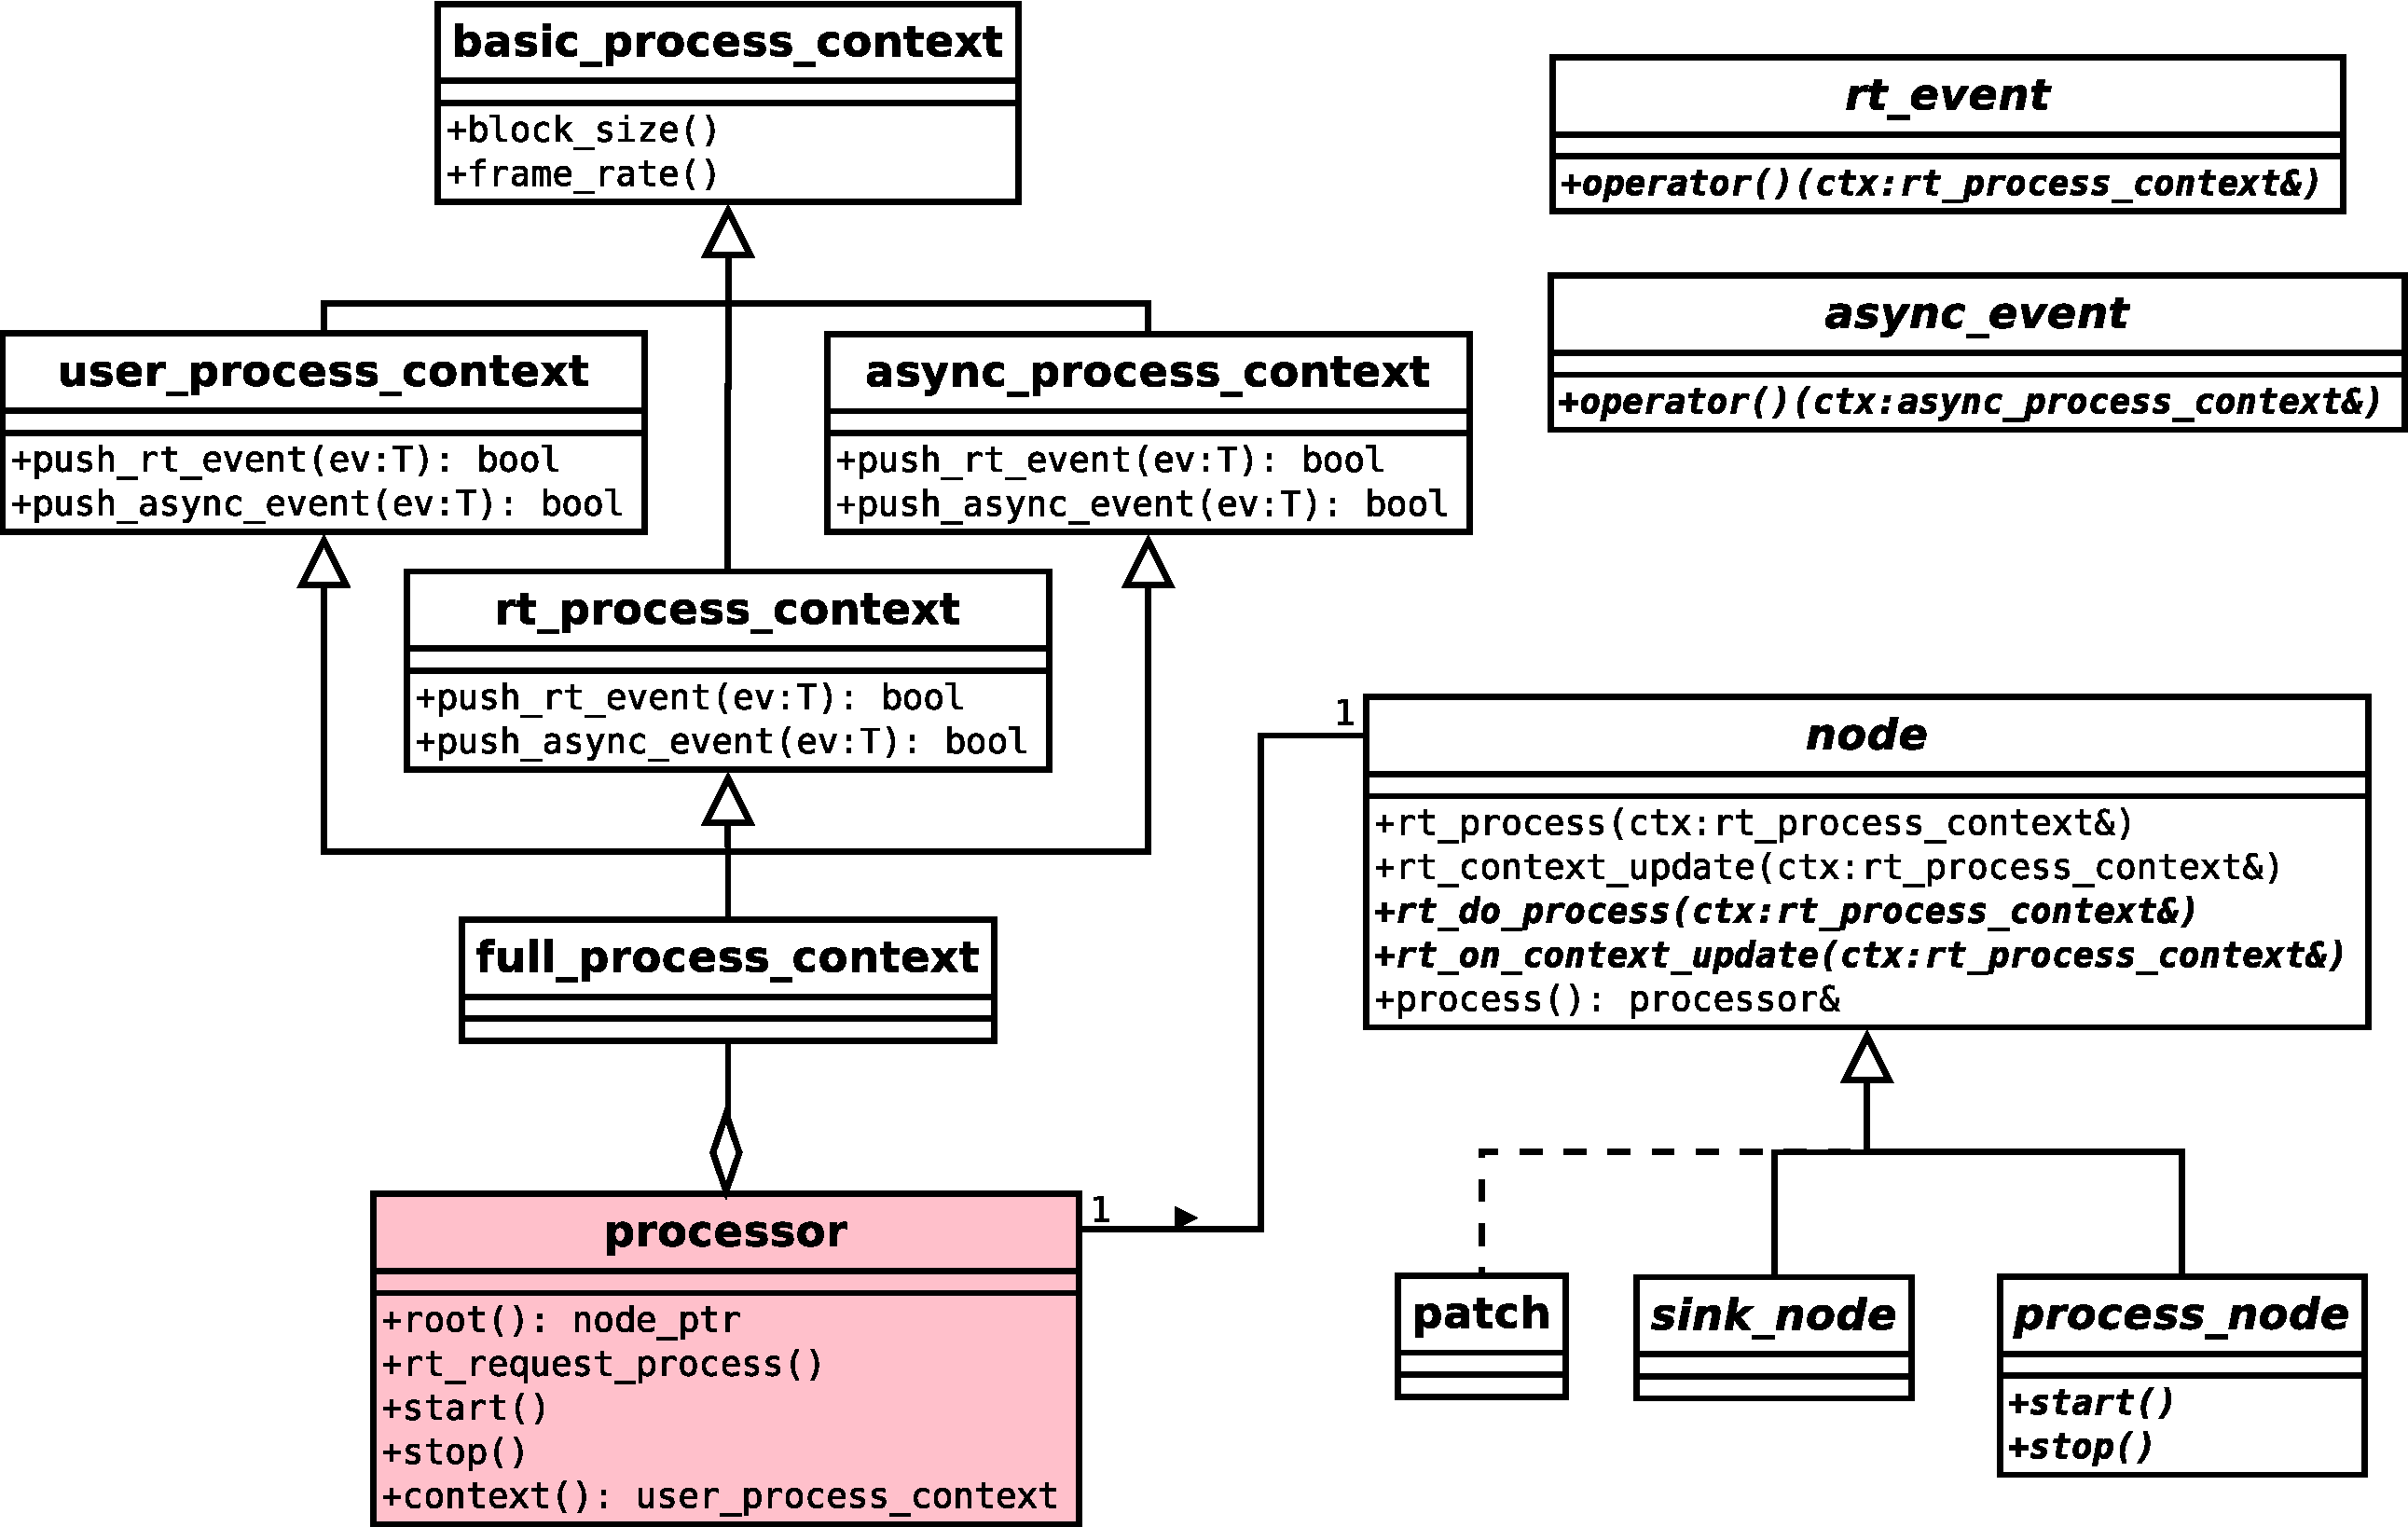
\includegraphics[width=\textwidth]{pic/graph-processor.pdf}
  \caption{The graph processor, its context and the processing methods
    of nodes. }
  \label{fig:graphprocess}
\end{figure}

Figure \ref{fig:graphprocess} introduces some new classes that are the
coordinate the execution of the synthesis graph. Because there are
several concurrent ---and potentially parallel--- threads of
execution, writing code without race conditions and other
synchronisation problems can get quite hard if we do not establish
some conventions. Unless otherwise specified in its documentation, a
method is expected to be executed in only one \emph{kind} of thread,
sometimes even in just only one specific thread. There are three kinds
of threads and some naming conventions allow us to determine in which
thread some method is expected to be used:

\begin{description}
\item[User thread] The user thread is the one where most objects are
  created and where usually the user interface lives. In some way,
  this can be considered the \emph{normal thread}, and it is the root
  of the thread tree --- i.e. the one that creates the other threads.

  If a method does not have any special prefix nor belongs to a class
  named with a special prefix, we shall assume, unless otherwise
  specified in its documentation, that it is safe to execute it only
  in the user thread. In the current implementation, these methods,
  while reentrant, they are not fully thread-safe. This means that
  most non-const methods of an object and related objects
  ---i.e. objects that keep references among themselves--- shall be
  executed in the same thread, but it is safe to operate with
  unrelated objects in different user threads.

\item[Real-Time (RT) threads] These are the threads where the actual
  work of processing the synthesis graph is done. As we shall see
  later, these threads are controlled by the \type{process\_node}
  derivates, but that is not relevant now. Methods beginning by the
  \type{rt\_} prefix, and all methods of classes named with that
  prefix, are expected to be executed in this thread. While it can be
  normal for several RT threads to coexist, implementers of RT-methods
  and objects should not worry about this, because, unless they are
  actually implementing a \type{process\_node}, the system itself
  serialises calls to dependent methods --- in the current
  implementation, it just serialises calls to
  \type{rt\_request\_process}, we will discuss this soon.

\item[Asynchronous operation threads] These threads, that we
  may call just \emph{async threads}, ease the execution of operations
  that are forbidden in the RT thread. The \type{processor} controls
  the execution of these threads. Methods and classes prefixed with
  \type{async\_} are expected to be executed in these thread.
\end{description}

\subsubsection{Processing the graph}

The \type{processor} class is a \emph{fecade} that manages the
execution of the synthesis graph described by a given root node. Of
course, a whole graph can be attached to one and only processor and an
exception would be thrown if we try to attach it to several.

\begin{algorithm}
  \caption{Process a control iteration of the graph, $rt\_process (n,
    ctx)$}
\label{alg:processgraph}
\begin{algorithmic}
  \REQUIRE $\;$\\
  $n \in \mbox{\type{node}}$ \\
  $ctx \in \mbox{\type{rt\_process\_context}}$
  \ENSURE $\;$\\Every node in the graph is processed and its results ready in their
  outputs, if any, in the right order.
  \medskip
  \IF{$\lnot visited (n)$}
  \FORALL{$i \in inputs (n)$}
  \IF{$connected (i)$}
  \STATE $n_i \gets source (i)$
  \STATE $rt\_process (n_i, ctx)$
  \ENDIF
  \ENDFOR
  \STATE $rt\_do\_process (n, ctx)$
  \STATE $visited (n) \gets \top$
  \ENDIF
\end{algorithmic}
\end{algorithm}

The \type{rt\_request\_process} method triggers the execution of one
iteration of the graph, this is, it processes one block of audio rate
samples or one control sample. The processing algorithm is as
follows. The processor keeps a list the nodes that have side-effects
outside the graph itself, for example, an node for outputting to a
device. These are the nodes that inherit from \type{sink\_node}, and
we can refer to them as just \emph{sinks}. For every sink, the
processor invokes the recursive algorithm \ref{alg:processgraph}
implemented by \type{rt\_process} in the \type{node} class. This
recursively calls the process method of the nodes connected to one's
input. Because the synthesis graph may have loops and input ports may
be connected to several outputs, it marks every node it visits. In
this way, every node is processed only once and nodes that may have no
side effects are discarded --- because they do not interact wit the
``real world'' nor any node that does depends on it. When a node is
being visited, the pure virtual \type{rt\_do\_process} methods is
invoked. That is the most important method that implementers of
their DSP modules have to take care of; in it they should fetch the
input data, if any, process it, and write some output, if any. We
often just call this the \emph{worker method} of a node.

\subsubsection{Proactive nodes}

\type{rt\_do\_process} is usually executed by implicitly triggered by
\emph{process\_nodes}. These nodes represent devices that may require
processing from the graph have and extra \type{start ()} and
\type{stop ()} method. They are in charge of managing their own thread
where they request processing whenever they need frames.

A canonical concrete \emph{process\_node} is
\emph{core::async\_output}, which, when associated to an asynchronous
output device (see section \ref{sec:asyncio}), requests processing in
the output callback and passes what it gets from its single input port
to the device. In order to allow several asynchronous output devices,
calls to \type{rt\_request\_process} are serialised. Then, in their
worker method they just accumulate their input in an internal ring
buffer, but not directly output to the device, because that operation
may block and delay other devices that are waiting on this request. In
their own device callback, when there is enough information in their
internal ring buffer, this is sent to the device.

Calls to \type{rt\_request\_process} are serialised using a mutex in a
special way. When we try to get the lock and is owned already, we do
wait for the ongoing request to finish, but we do not perform a new
request, because the one that was already on the way might have been
enough for the device to get sufficient information. This use of locks
does not violate the RT rules, because all threads that are expected
to contend for it are real-time so no priority inversion can occur. It
may introduce some context switches, but that is unavoidable, and in
practise they do not add much overhead, and in modern processor the
gained parallelism compensates. While we are doing the output
operation on the device, another process node might have triggered
another request, preparing our next bunch of frames already. When we
are locked on the mutex, another RT thread is already doing what we
wanted to do, and if the OS scheduler is not dumb, it should preempt
our RT thread soon at it will happily find that its request have been
processed already. Thanks to this mechanism we can output to several
devices at the same time, even if they are in different sound
cards. What is output to each one depends on how the graph is
interconnected, and it might even be different. This is a common
usecase, for example, DJ's peek at how it the next track mix's in
while they adjust its tempo on their headphones without altering what
is still being played on the loudspeakers. Figure \ref{fig:djscheme}
shows how a typical DJ setup could be built with Pyschosynth's engine
and illustrates the most important aspects of the algorithm that we
just described.

\begin{figure}[h!]
  \centering
  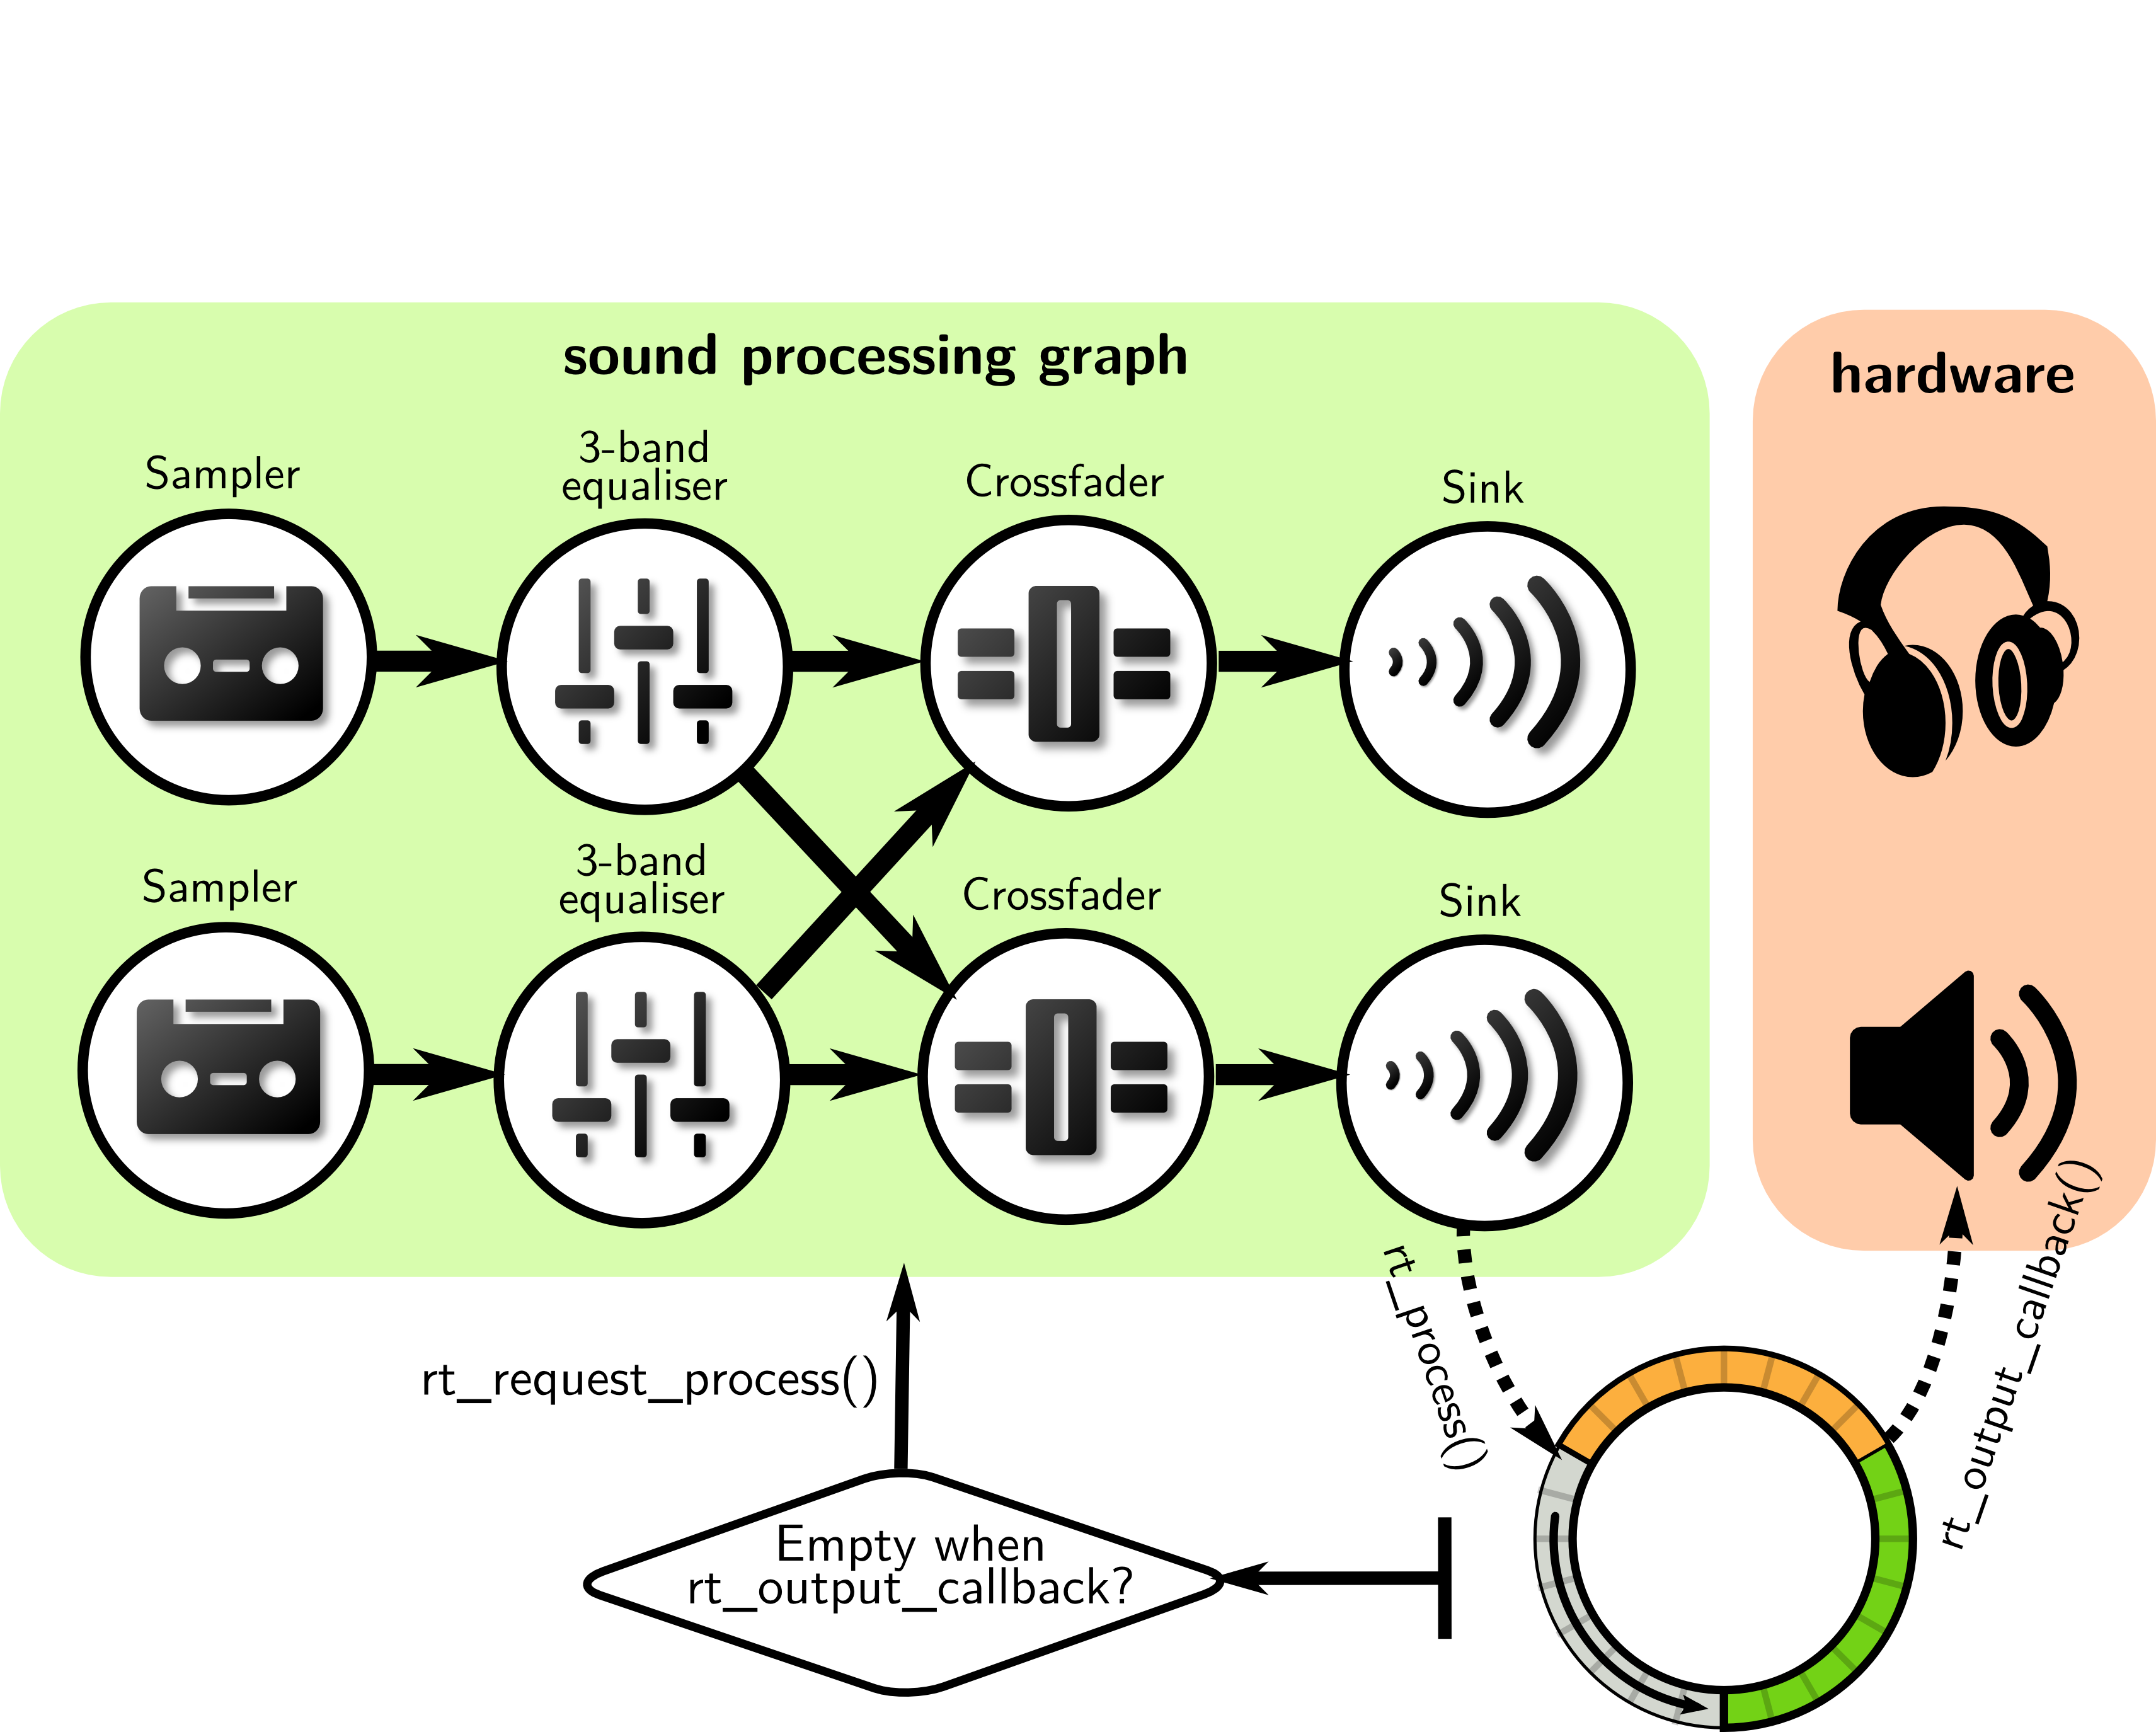
\includegraphics[width=\textwidth]{pic/djscheme.png}
  \caption{A DJ setup built with Psychosynht's engine to illustrate the multiple device output system.}
  \label{fig:djscheme}
\end{figure}

The \type{start ()} and \type{stop ()} methods in the \type{processor}
class is in charge of starting and stopping all the process nodes in
its associated graph. It also starts nodes that are added after the
processor have already been started and stops them when
removed. Usually, we can just start the processor at the beginning of
our program and start manipulating its graph. These methods also
control the execution of the \emph{async thread}. 

For completeness, we shall mention that there are exists passive
output nodes that only write data in the event of an external request
for processing. We can use this, for example, to record a live session
driven by a second active device to a file. Also, if we only want to
generate the audio directly in the file without the presence of any
proactive sink, we may directly call \type{rt\_process\_request} in
the user thread as many times as needed, taking into account that the
duration of the file resulting from calling it $i$ times is, in
seconds:
\begin{equation}
  duration(i) = \frac{i \times block\_size}{frame\_rate}   
\end{equation}

\subsubsection{Communication between threads}

Creating proper abstractions for communicating among the different
threads is essential for the extensibility of the system. This is, in
fact, one of the main flaws of the former implementation of this
layer; the usage of ad-hoc mechanisms for every different feature made
the system harder to understand, leading to subtle race conditions,
the overuse of locks and unnecessary busy-wait alike checks in the RT
thread.

It should be almost clear already why we need our own thread
communication abstraction instead of just using some traditional
blocking mechanism --- message passing, monitors, etc. First, the RT
threads should not wait on non-RT threads like the user thread or the
async threads. Moreover, most of the processing in the RT thread
should be done in tight, simple, loops; even if the parameters coming
from other threads where implemented with atomic variables, this state
should not change during the execution of these loops. What we do
instead is to delegate the execution of actions with side-effects
visible by another thread to that thread itself. We call these actions
\emph{events}, and they are an instance of the \emph{command} design
pattern \cite{gamma95design}. Going back to figure
\ref{fig:graphprocess}, we can distinguish two kinds of events,
\type{rt\_event}, that are to be executed by the RT thread, and
\type{async\_event}, that are executed in the asynchronous
thread. Note that there is no notion of \type{user\_event}, because
that would add unnecessary complexity. If the async thread wants to
produce side-effects visible to the user, they can just coordinate
using locks, because they are not forbidden in the async thread. If
the RT thread wanted to do so, he can just send an event to the
asynchronous thread that does the synchronised update in that
unconstrained environment.

The events are just functors with its overloaded \type{operator()}
virtual. The \emph{fn\_*\_event} family of concrete events just wrap a
non-polymorphic functor to match the corresponding interface. This
recurring pattern of embedding a object with a non-polymorphic
interface into an adaptor with the same interface implemented with
virtual methods is called \emph{boxing}. The \type{make\_*\_event}
family of box factories use template argument deduction to
automatically box its parameter without explicitly writing its
type. This is extremely useful with the new C++11 lambdas, because to
have a compile-time determined size\footnote{Something that gracefully
  allows us to use them even in our RT-thread as long as we do not
  erase its type with a \type{std::function<>}}, every lambda
expression has a distinct, anonymous, compile-time determined type
\cite{jarvi10lambda}. Using lambda expressions to create events rises
the conciseness and clarity of the code, because the code that
asynchronously produces the side-effects follows directly to the
source of this event. If you are eager to see this pattern of control
flow abstraction in use, skim to example \ref{lst:nodeexample1}.

The events are stored inside the \emph{process context}. This is where
the common information that characterises the processing is stored,
such as the block size or the sample rate. Also the event deques are
stored there. The \type{basic\_process\_context} holds all this
information. But, instead of directly exposing access to the event
queues, three classes that virtually inherit from it offer different
access methods for them, even though with the same signatures. These
are the \type{user\_process\_context}, \type{rt\_process\_context} and
\type{async\_process\_context}. Each event deque is split in a
triple-buffer fashion. Which internal buffer should we push events in,
and what kind of lock, if any, should we use when doing so, depends on
the thread that is the source of the event. These three views on the
process context manage this implementation logic transparently to the
user. We designed our API carefully to ensure that the code executed
in each process has access only to the proper view of the context; in
this way, the type system ensures that events are sent in the right
way, giving confidence to the programmer about his own code.

The events received in the RT thread from other threads are processed
at the beginning of each \type{rt\_request\_process} just before
executing the synthesis graph. Events that are sent from the RT thread
to the RT thread itself are instead processed at the end of the
request. Recursive events are delayed to the next request. Events are
accumulated and sent in blocks, in this way we avoid the unlikely
situation in which the user thread is constantly sending events, the
RT thread processes them, and never advances to execute the synthesis
graph.

\label{fig:triplebuf}
The async thread is in an infinite loop waiting to receive and process
events. Once again, it receives events from the RT thread in blocks
that are dispatched at the end of every RT process cycle.

There two triple-buffer structures, one associated to the RT thread
and another one for the async thread. Each triple buffer contains
three \type{hetero\_deques}\footnote{The interested reader can take a
  look at the \type{graph::triple\_buffer} class, which is
  parametrised over the buffer type and the synchronisation policy for
the ``flip'' operations.} where one can push events of any derivate of
the \type{rt\_event} and \type{async\_event} respectively. Multiple
buffering is a technique often associated to computer graphics. Each
buffer is accessed through a pointer; one part of the system is
writing data from one of the buffers (the back buffer) and another one
is concurrently reading from another (the front buffer). When the
reader is done with the current a simple pointer swap operation
(called the buffer ``flip'') feeds him with a bunch of new information
coming from the back buffer, and the writer gets a new fresh blank
buffer where to dump new data. The three buffers associated to each of
our triple-buffer structures have the following semantics, as
exemplified by figure \ref{fig:triplebuf}:

\begin{figure}[h!]
  \centering
  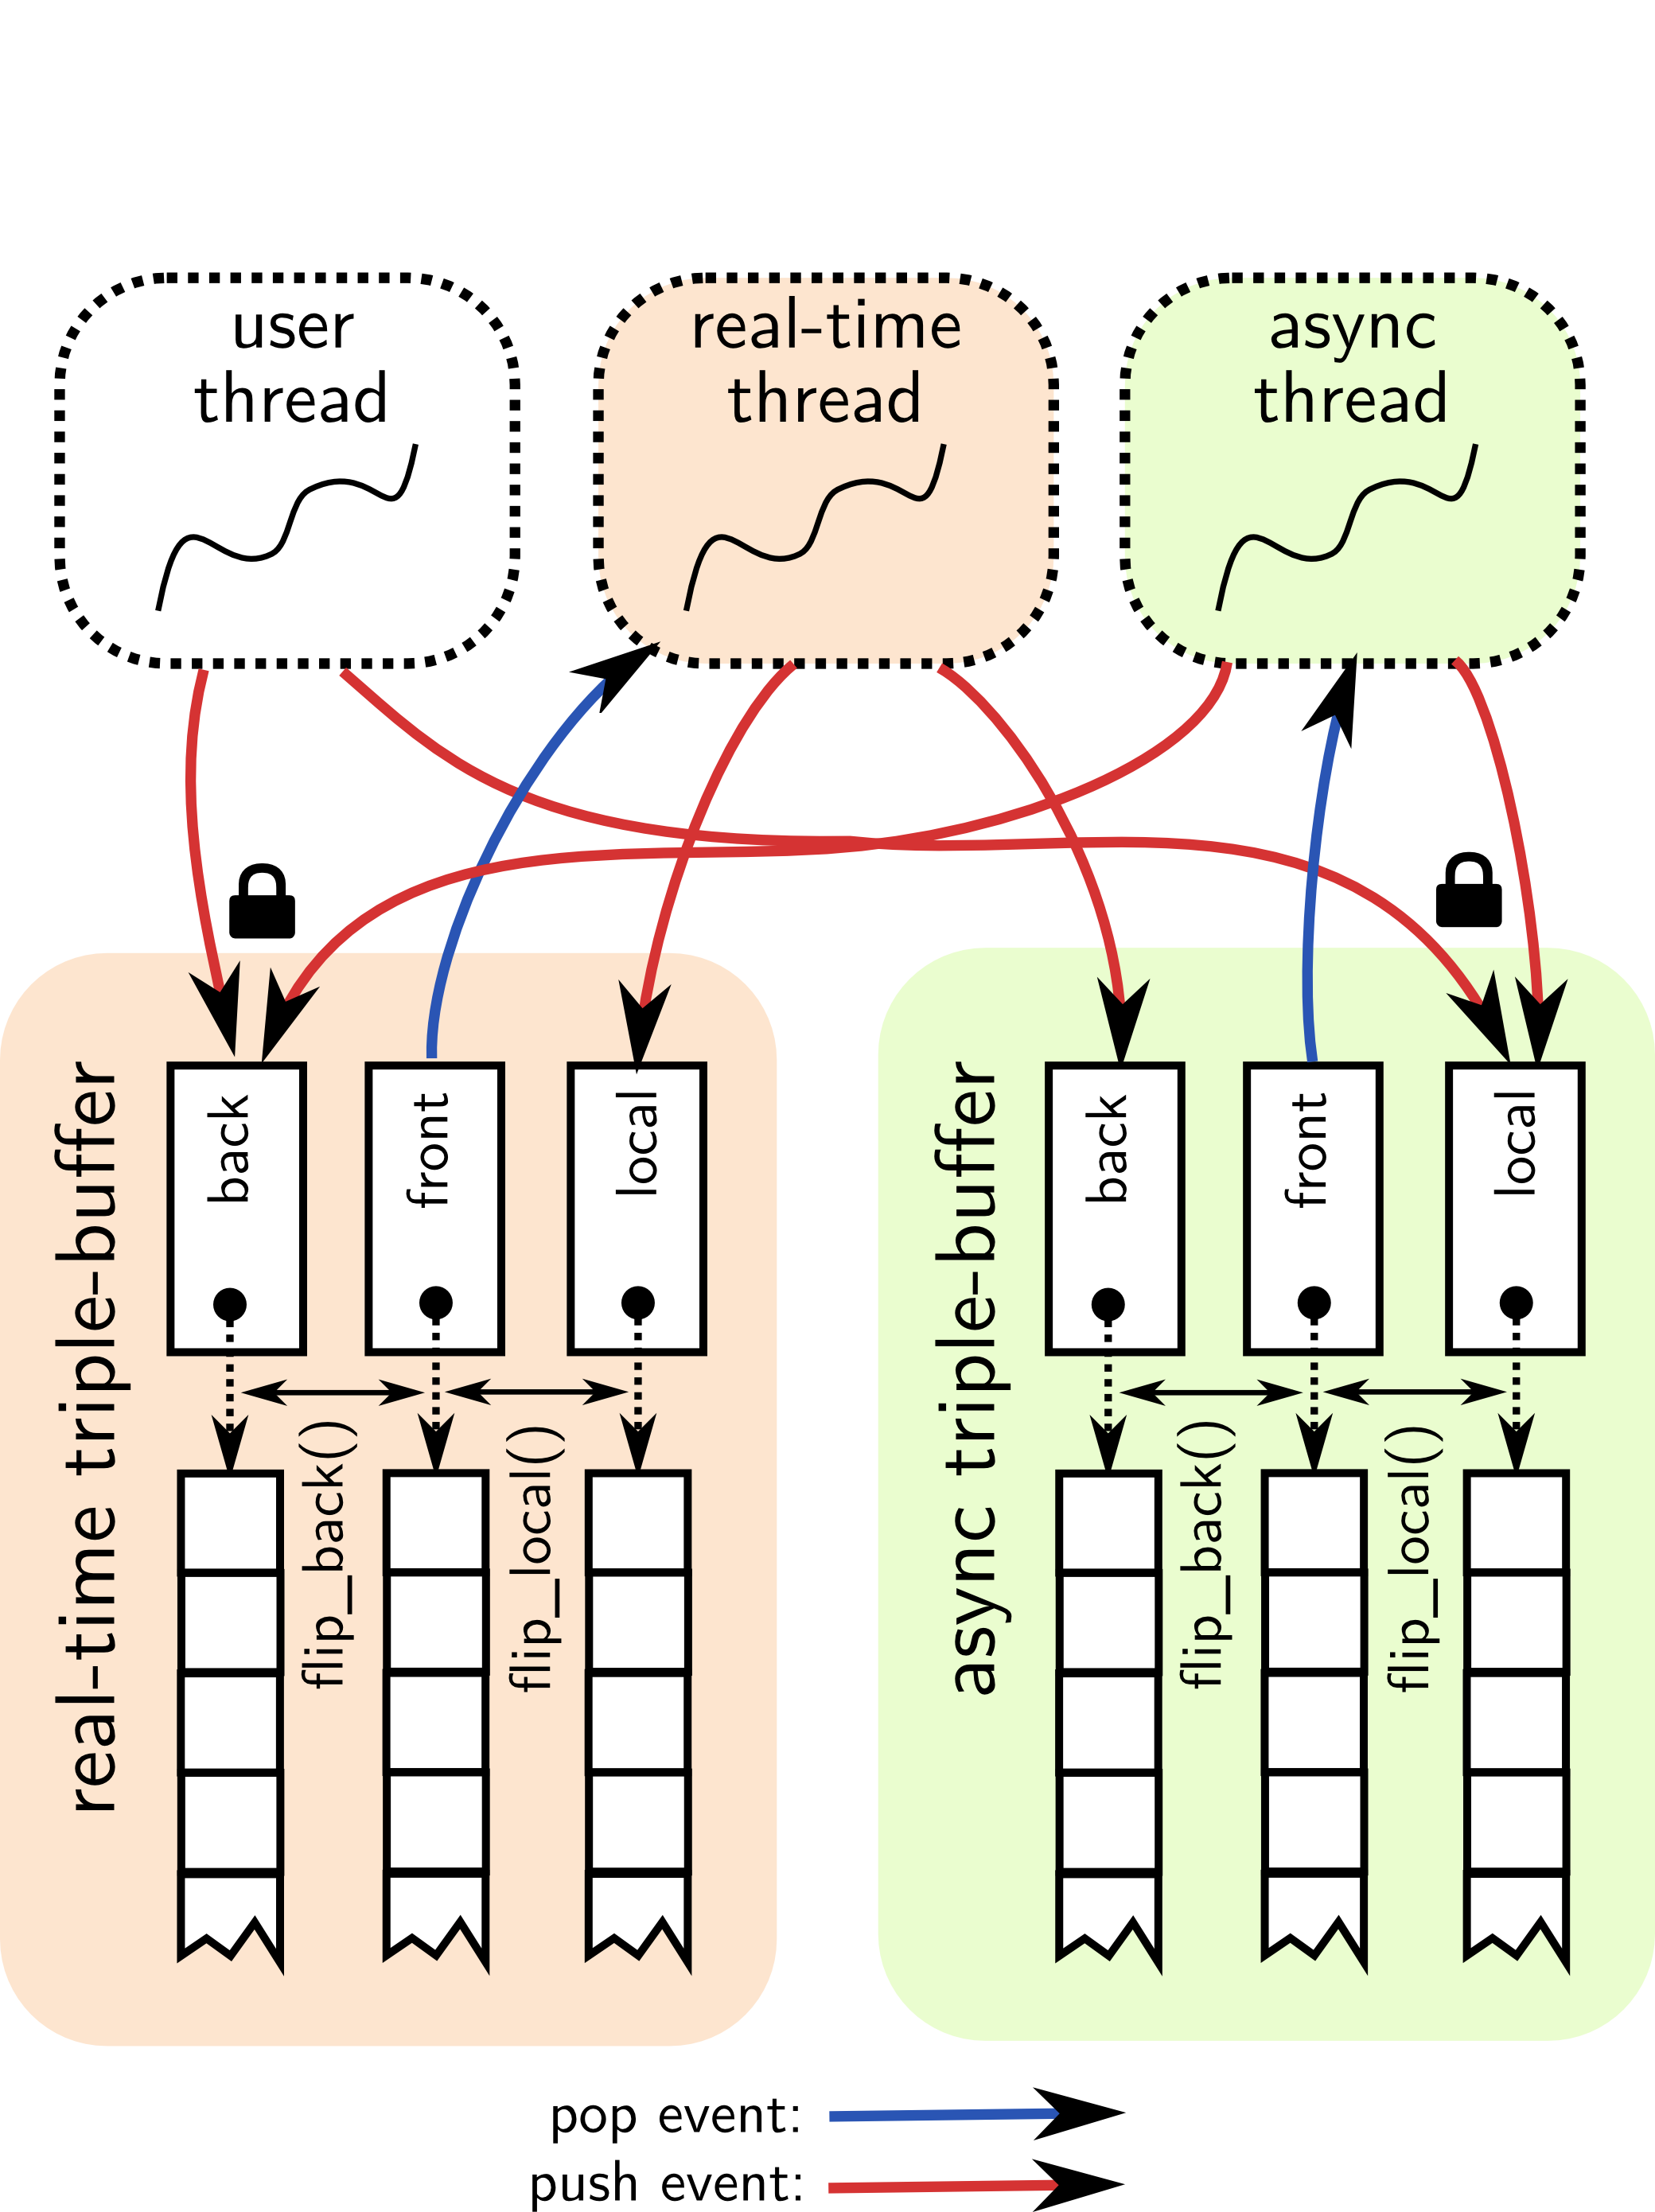
\includegraphics[width=\textwidth]{pic/events.png}
  \caption{Communication with triple buffer event deques.}
  \label{fig:triplebuf}
\end{figure}

\begin{description}
\item[Front buffer] This is the buffer where the events are popped
  from for processing. Only the RT thread should access the front
  of its triple buffer, and the same happens in the async thread.

\item[Back buffer] This is, in general, the buffer where events coming
  from other threads are written to. In the RT triple buffer case, the
  both the user thread and the async thread do write into it, but they
  synchronise their insertions with a mutex --- because they can! The
  \type{flip\_back ()} method exchanges the front and back
  buffers. The flip is done in the RT thread, at the beginning of each
  process request, thus should can not contend for the mutex. Instead
  it does a conditional lock, and if it fails, it skips the flip. This
  may lead to some events to be delayed more than one request if there
  is a lot of contention on the mutex --- i.e. the user and async
  threads are writing a lot of events --- but that does not happen in
  practise and informal experiments suggest that the approach is
  enough. However, this could be completely solved by implementing
  \type{hetero\_deques} lock-free at least for one writer and one
  reader, we develop this idea in section \ref{sec:improvehetero}. In
  that case, the user and async thread would still need to serialise
  their writes, but the RT can flip and read safely without caring
  about the mutex at all.

  The back of the async triple buffer is slightly different. Here,
  only the RT thread writes, because if the user thread could write on
  it at the same time we would need a lock. Indeed, it is also the RT
  thread who does the flip after filling it, as long as the async
  thread is not still processing the current front buffer, otherwise
  the flip is postponed.

\item[Local buffer] The local buffer is where a buffer writes events
  that he sends to itself. Thanks to this, we can have a notion of
  ``post-processing'' and also infinitely recursive events that
  generate a new event each time; this is very useful for implementing
  tasks and state machines. If a thread wrote his own events in its
  front buffers, this kind of behaviour would lead to an infinite loop
  and events sent to the back buffer would never be processed. The
  \type{flip\_local ()} method exchanges the front and local buffers.

  Note that in the local buffer of the async thread is a bit
  special. Because the RT thread has exclusive non synchronised access
  to the back buffer, events from the user thread are sent to the
  async thread through the local buffer, and they use a mutex to avoid
  data races.
\end{description}

While this structure might seem a bit baroque, all the complexity is
hidden in the \type{processor} and \type{*\_process\_context}
classes. In most cases, one should only care about making the right
choice of which thread should execute our event; all the complexity of
delivering and processing it is hidden and the type system ensures
we can only do it in a thread safe way.

Listing \ref{lst:nodeexample1} show an example on how to use this
event passing system. The frequency parameter is set from the user
thread, but it must be read from the RT thread and the related
variable \emph{dt} must be updated. Doing this in a portable and
thread-safe way without using mutexes is tricky. Thanks to our
structure, we just send an event that does the job of updating the
variables. There are no possible data races even if reading/writing
float values is not atomic, because the lambda expression captures a
local copy of the \type{freq} variable. This is a very convenient
fact: the event's own state provides an intermediate buffer for
communicating value updates without data races; the lambda semantics
in C++0x just provides us the syntactic sugar to make the code
pleasant to write and read. Please remember that this code is here
only to illustrate the usage of the event passing system; in practice,
passing parameters from the user thread to the RT thread is even
simpler, as we will explain in section \ref{sec:graphcontrols}.


\begin{lstlisting}[float=h, label=lst:nodeexample1, caption=A thread communication use-case]
struct example_oscillator_node : public node
{
    example_oscillator_node ()
        : _freq (440.0f) , _rt_freq (_freq), _rt_phase (0)
        , _rt_dt (0) // rt_on_context_update will be executed before
                     // the first process so we can set properly this
                     // variable that depends on the frame rate.
    
    void set_frequency (float freq) {
        _freq = freq;
        auto& ctx = process ().context ();
        ctx.push_rt_event (make_event ([=] (rt_process_context& ctx) {
            _rt_freq = freq;
            _rt_dt   = 1 / (freq * ctx.frame_rate ());
        }));
    }
    float frequency () const
    { return _freq; }

protected:
    void rt_on_context_update (rt_process_context& ctx)
    { _rt_dt = 1 / (_rt_freq * ctx.frame_rate ()); }

    void rt_do_process (rt_process_context& ctx) {
        auto frames = ctx.block_size ();
        while (frames --> 0) {
            // We suppose M_PI is defined. The output_sample function
            // does not actually exist, it is just an example.
            output_sample (std::sin (_rt_phase * 2 * M_PI));
            _rt_phase += dt;
        }
    }

    float _freq, _rt_freq;
    float _rt_phase, _rt_dt;
}
\end{lstlisting}

\subsection{Indirect object construction}

\label{sec:graphfactory}
\label{sec:modports}

\section{Validation}

\section{Conlusion}

%%% Local Variables: 
%%% mode: latex
%%% TeX-master: "00-main"
%%% End: 
